\documentclass[11pt]{article}
\usepackage[T1]{fontenc}
\usepackage[utf8]{inputenc}
\usepackage{lmodern}
\usepackage[margin=1.05in]{geometry}
\usepackage{amsmath,amssymb,amsthm,mathtools}
\usepackage{microtype}
\usepackage{booktabs,longtable,array}
\usepackage{enumitem}
\usepackage{xcolor}
\usepackage{tikz}
\usetikzlibrary{patterns}
\usepackage{listings}
\usepackage{needspace}
\usepackage[unicode,hidelinks]{hyperref}
\hypersetup{pdftitle={A finite-time singularity of Calabi flow on projective space},pdfauthor={OpenAI}}
\ifdefined\pdfinfoomitdate\pdfinfoomitdate=1\fi
\ifdefined\pdftrailerid\pdftrailerid{}\fi
\ifdefined\pdfsuppressptexinfo\pdfsuppressptexinfo=-1\fi
\numberwithin{equation}{section}
\newtheorem{theorem}{Theorem}[section]
\newtheorem{proposition}[theorem]{Proposition}
\newtheorem{lemma}[theorem]{Lemma}
\newtheorem{corollary}[theorem]{Corollary}
\theoremstyle{definition}
\newtheorem{definition}[theorem]{Definition}
\theoremstyle{remark}
\newtheorem{remark}[theorem]{Remark}
\newcommand{\CP}{\mathbb{CP}}
\newcommand{\R}{\mathbb{R}}
\newcommand{\C}{\mathbb{C}}
\newcommand{\N}{\mathbb{N}}
\newcommand{\Z}{\mathbb{Z}}
\newcommand{\A}{\mathcal A}
\newcommand{\Pcal}{\mathcal P}
\newcommand{\Dcal}{\mathcal D}
\newcommand{\wt}{\widetilde}
\newcommand{\wh}{\widehat}
\newcommand{\dd}{\mathrm{d}}
\newcommand{\e}{\mathrm{e}}
\newcommand{\eps}{\varepsilon}
\newcommand{\ip}[2]{\langle #1,#2\rangle}
\newcommand{\norm}[1]{\lVert #1\rVert}
\newcommand{\abs}[1]{\lvert #1\rvert}
\DeclareMathOperator{\supp}{supp}
\DeclareMathOperator{\spec}{spec}
\DeclareMathOperator{\diag}{diag}
\setlist[enumerate]{itemsep=3pt,topsep=5pt}
\setlist[itemize]{itemsep=3pt,topsep=5pt}
\setlength{\emergencystretch}{1.5em}
\lstdefinestyle{certificate}{language=Python,basicstyle=\ttfamily\footnotesize,
  numbers=left,numberstyle=\tiny\color{black!60},numbersep=7pt,
  breaklines=true,breakatwhitespace=false,columns=fullflexible,
  keepspaces=true,showstringspaces=false,tabsize=4,
  keywordstyle=\bfseries,commentstyle=\itshape\color{black!65},
  frame=single,framerule=.3pt,xleftmargin=1em,xrightmargin=.2em,
  aboveskip=1em,belowskip=1em,
  literate={²}{{$^2$}}1 {≤}{{$\le$}}1}

\title{A finite-time singularity of Calabi flow\protect\\ on projective space}
\author{OpenAI}
\date{September 24, 2026}
\begin{document}
\maketitle
\begin{abstract}
We construct a smooth K\"ahler metric in the Fubini--Study class of
\(\CP^{10}\) whose Calabi flow develops unbounded scalar curvature in finite time.
This disproves Chen's smooth long-time existence conjecture, even in a class
containing a constant-scalar-curvature metric.
\end{abstract}
\section{Introduction}\label{sec:introduction}
Let \(\omega_0\) be a smooth K\"ahler form on a compact complex manifold \(M\).
We use the scalar-curvature convention
\(S(\omega)=\operatorname{tr}_\omega\operatorname{Ric}(\omega)\).
The Calabi flow is
\begin{equation}\label{eq:calabi-flow}
 \omega(t)=\omega_0+i\partial\bar\partial\phi(t)>0,
 \qquad \phi(0)=0,\qquad
 \partial_t\phi=S(\omega(t))-\bar S,
\end{equation}
where \(\bar S\) is the average scalar curvature, determined by the K\"ahler class.
Calabi introduced this flow to seek canonical metrics within a K\"ahler
class~\cite{Calabi1982}. Chen's smooth long-time existence conjecture
asserts that the flow exists for all positive times from arbitrary smooth
K\"ahler initial data; see \cite[Conjecture~1.1]{HeZeng2021}.
We give a counterexample on projective space. Write
\(\omega_{\mathrm{FS}}\) for the Fubini--Study form whose potential
on the standard affine chart is \(\log(1+|Z|^2)\).

\begin{theorem}\label{thm:main}
There is a smooth \(U(10)\)-invariant K\"ahler form \(\omega_0\) on
\(\CP^{10}\), in the class \([\omega_{\mathrm{FS}}]\), whose maximal smooth
Calabi flow has existence interval \([0,T_*)\) with \(0<T_*<\infty\).
There are a point \(p\in\CP^{10}\) and a constant \(a>0\) such that
\[
 S(\omega(t))(p)\sim a(T_*-t)^{-1/2}\qquad\text{as }t\uparrow T_*.
\]
\end{theorem}

The Fubini--Study metric has constant scalar curvature. Thus the example
also answers negatively the smooth global-existence question for classes
containing a constant-scalar-curvature K\"ahler metric, emphasized by
Chen and Cheng~\cite[p.~912, following Conjecture~1.3]{ChenCheng2021}.
In particular, no assertion of smooth global existence and subsequent
smooth convergence modulo holomorphic automorphisms can hold for arbitrary
smooth initial metrics in such a class: the obstruction already occurs
at a finite time.

The same singularity persists on products with a stationary factor.
\begin{corollary}[Products with stationary factors]\label{cor:product-singularities}
Let \(\omega(t)\), \(T_*\), \(p\), and \(a\) be as in
Theorem~\ref{thm:main}, and let \((Y,\eta)\) be a compact connected
K\"ahler manifold with \(\eta\) of constant scalar curvature.  With
\(\pi_X\) and \(\pi_Y\) the projections from \(\CP^{10}\times Y\),
the maximal smooth Calabi flow from
\(\Omega_0=\pi_X^*\omega_0+\pi_Y^*\eta\) is
\[
 \Omega(t)=\pi_X^*\omega(t)+\pi_Y^*\eta,
 \qquad 0\leq t<T_*.
\]
For every \(y\in Y\),
\(S(\Omega(t))(p,y)\sim a(T_*-t)^{-1/2}\).
In particular, finite-time smooth Calabi-flow singularities occur in
every complex dimension \(n\geq10\), on
\(\CP^{10}\times\CP^{n-10}\), in a class containing a
K\"ahler--Einstein metric.
\end{corollary}
The corollary is proved after Theorem~\ref{thm:main} in
Section~\ref{sec:compact}.

\subsection{Background and significance}
On compact Riemann surfaces, Chru\'sciel proved global forward existence
and convergence to a constant-curvature metric~\cite[Theorem~2.1]{Chrusciel1991}.
Chen gave a different proof using decreasing functionals and concentration
compactness~\cite{Chen2001}, and Struwe developed a unified treatment of
Calabi and normalized Ricci flows on closed surfaces~\cite{Struwe2002}.
In higher dimensions, Chen and He proved local existence and uniqueness
and established stability near a constant-scalar-curvature
metric~\cite[Theorems~1.2 and~3.2]{ChenHe2008}. He and Zeng developed
short-time theory for rougher initial metrics~\cite{HeZeng2021}.
These higher-dimensional results concern either short times or restricted
initial data.

Curvature estimates give continuation criteria for the smooth flow.
Chen and He proved extension under a uniform Ricci-curvature
bound~\cite[Corollary~5.3]{ChenHe2008}, and Chen and Cheng established
extension under a uniform scalar-curvature bound~\cite[Theorem~1.8]{ChenCheng2021}.
Li, Zhang and Zheng state that a uniform spatial $L^p$ scalar-curvature
bound, measured with respect to the evolving metric, suffices when
$p>\dim_{\C}M$~\cite[Theorem~1.2]{LiZhangZheng2024}; Li and Zhang
state a further criterion involving spacetime scalar and
scalar-Laplacian integrability~\cite[Theorem~1.1]{LiZhang2025}.

On a compact almost homogeneous manifold with two hypersurface ends,
Guan proved exponential smooth convergence of the modified Calabi flow
for initial metrics invariant under a maximal compact subgroup of the
automorphism group~\cite[Theorem~A]{Guan2007}.
The two special orbits of the action used here are instead a point and
the hyperplane at infinity. The point has complex codimension ten, so
the two-hypersurface hypothesis fails.

Streets constructed global weak Calabi flows by minimizing
movements~\cite{Streets2014}. Berman, Darvas and Lu identify these flows
with trajectories in a space of finite-energy K\"ahler potentials and show
that, when the class contains a constant-scalar-curvature metric, every
weak trajectory converges to a smooth constant-scalar-curvature potential
in the $d_1$ distance, the extension of the $L^1$ path-length distance on
smooth K\"ahler potentials~\cite[Section~6 and Theorem~1.11]{BermanDarvasLu2017}.
The weak and classical flows agree for as long as the latter exists
smoothly~\cite[Proposition~6.1]{BermanDarvasLu2017}.
Neither this weak continuation nor the large-time $d_1$ convergence implies
smooth continuation through every finite time.

\subsection{Structure of the construction}

The construction first reduces the flow to a scalar equation, then builds
an exact shrinking solution of its flat limit, and finally corrects that
solution on the compact manifold. The geometric starting point is the
radial ansatz of Calabi~\cite{Calabi1979} and the momentum formulation
of Hwang and Singer~\cite{HwangSinger2002}. Abreu's toric
scalar-curvature formula~\cite{Abreu1998} is expressed in Guillemin's
symplectic-potential framework~\cite{Guillemin1994}.
For a radial potential \(\Phi(\ell)\), where
\(\ell=\log|Z|^2\), set \(x=\Phi'(\ell)\) and
\(v=\Phi''(\ell)\). We use \(x\in(0,1)\) as the momentum
coordinate and write
\[
 v=x(1-x)+x^2(1-x)^2H.
\]
Smoothness and positivity at both special orbits are encoded by
\(H\in C^\infty[0,1]\) and \(1+x(1-x)H>0\).
Section~\ref{sec:geometry} derives the scalar fourth-order equation
for \(H\), including the affine choice in the Legendre potential
needed to recover the Calabi flow with its prescribed normalization.
It also realizes the fixed spatial operator on an auxiliary sphere,
where the endpoint conditions become ordinary smooth invariance.

The singularity is detected by one value of \(H\). At the fixed
affine origin \(p\), the scalar-curvature identity is
\[
 S(t,p)=110\bigl(1-H(t,0)\bigr).
\]
We construct a smooth positive profile \(G\), bounded above and away from
zero, with \(G(0)=1\) and \(G'(0)<0\), and set
\[
 F(t,x)=\rho^{-1}h(x/\rho),\qquad
 h(y)=\frac{G(y)-1}{y},\qquad
 \rho=\sqrt{-t},\quad t<0.
\]
Then \(F(t,0)=\rho^{-1}G'(0)\). Our task is to find an exact
compact solution \(H=F+V\) for which positivity persists and
\[
 V(t,0)=O(\rho^{-1+\delta})\qquad\text{for some }\delta>0.
\]
The correction is therefore smaller than the leading term at the
origin, preserving the desired scalar-curvature divergence. A smooth
interior time slice of this solution will be the initial metric;
no initial metric needs to be fixed before the construction.

Section~\ref{sec:profile} constructs \(G\) so that \(F\) solves the
scale-invariant flat equation exactly. The profile is obtained by
matching a two-parameter analytic solution at the origin to a half-line
solution approaching a positive constant.
A finite exact-arithmetic calculation, with analytic enclosure and
nonlinear error bounds, certifies the matching inequalities. This uses
the framework of validated Taylor integration surveyed
in~\cite{NedialkovJacksonCorliss1999}.
The finite argument and its complete executable certificate appear in
the appendices. The resulting profile also has a differentiable
expansion at infinity; this expansion controls the compact error away
from the shrinking core.

The correction begins with a right inverse for the flat linearized
equation. Section~\ref{sec:parabolic} introduces the weighted norms
and local estimates, and Section~\ref{sec:flat} constructs this inverse
on all negative times. In similarity variables its time-one evolution
is a compact perturbation of a damped constant-coefficient evolution.
A spectral split determines finitely many components from future
forcing. This choice is available because the initial metric is still
free; it requires no stability or nondegeneracy theorem for the
profile. The compact-perturbation and spectral-projection tools are
classical~\cite{Kato1995}. After selecting a spectral weight, an outer
annulus estimate upgrades the temporal supremum bound to the full
spatially weighted parabolic H\"older estimate. The decisive input
there is a scale-invariant \(L^2\) bound that is integrable up to
the singular time.

Section~\ref{sec:compact} combines this ancient inverse near the core
with a short-time forward solution outside it. The outer forcing
cancels the inner cutoff commutator exactly; the remaining operator
errors are small. For the nonlinear correction one further needs the
compact residual to become small after applying the inverse. This
holds in a norm controlling all four spatial derivatives and their
temporal H\"older seminorms, with the time derivative omitted.
The outer estimate uses a strictly higher H\"older exponent for the
source, and the fixed-point equation then supplies the missing time
derivative. Positivity and the pointwise correction bound above give
the geometric hypotheses needed to finish Theorem~\ref{thm:main}.

\section{The geometric reduction and the finite-time obstruction}
\label{geo:section}
\label{sec:geometry}

We use scalar curvature in the convention
\(S(\omega)=\operatorname{tr}_{\omega}\operatorname{Ric}(\omega)\).
Let \(\omega_*\) be the Fubini--Study form on \(\CP^n\) with affine
potential \(\log(1+|Z|^2)\).  The geometric identities below hold for every
\(n\geq1\); the construction will use \(n=10\).
The radial and momentum descriptions follow the framework of
Calabi~\cite{Calabi1979} and Hwang--Singer~\cite{HwangSinger2002};
the Legendre-coordinate viewpoint is also central to the toric formulas
of Guillemin and Abreu~\cite{Guillemin1994,Abreu1998}. We give the
identities directly to fix the scalar convention and to verify
smoothness at the point orbit as well as at the divisor.
Set
\begin{equation}\label{geo:reference}
 q=|Z|^2,\qquad \ell=\log q,\qquad
 v_*(x)=x(1-x),\qquad w(x)=x^{n-1}.
\end{equation}
For a radial potential \(\Phi(\ell)\), its momentum coordinate and
momentum profile are
\[
 x=\Phi'(\ell),\qquad v(x)=\Phi''(\ell).
\]
The Legendre transform \(u(x)=x\ell-\Phi(\ell)\) satisfies
\(u'=\ell\) and \(u''=1/v\).  The reference transform is
\[
 u_*(x)=x\log x+(1-x)\log(1-x),\qquad u_*''=v_*^{-1}.
\]
Primes on functions of \(x\) will denote differentiation in \(x\).

\begin{proposition}[Exact fixed-class reduction]\label{geo:reduction}
Let \(I\) be an open time interval, and let
\(H\in C^\infty(I\times[0,1])\) satisfy
\begin{equation}\label{geo:positivity}
 b(t,x):=1+v_*(x)H(t,x)>0.
\end{equation}
Define
\begin{equation}\label{geo:momentum}
 v=v_*+v_*^2H=v_*b,\qquad
 K(H)=w^{-1}(wv_*^2H)'',\qquad
 \A H=\big[w^{-1}(wv_*^2H)''\big]''.
\end{equation}
At each time these data, together with an affine choice in the Legendre
potential, determine a smooth \(U(n)\)-invariant K\"ahler form in
\([\omega_*]\).  Its scalar curvature and average scalar curvature are
\begin{equation}\label{geo:scalar}
 S(t,x)=n(n+1)-K(H)(t,x),\qquad \bar S=n(n+1).
\end{equation}
If, in addition,
\begin{equation}\label{geo:equation}
 H_t+(1+v_*H)^2\A H=0,
\end{equation}
then for any \(t_0\in I\) and any initial affine choice there is a smooth
family of these forms satisfying the Calabi flow exactly.  More
precisely, its global potential relative to \(\omega(t_0)\) satisfies
\begin{equation}\label{geo:potential-flow}
 \phi(t_0)=0,\qquad
 \omega(t)=\omega(t_0)+i\partial\bar\partial\phi(t),\qquad
 \phi_t=S(\omega(t))-\bar S.
\end{equation}
\end{proposition}

\begin{proof}
We first verify smoothness and positivity at both endpoints.  Suppress
time for this part of the argument.  Since
\begin{equation}\label{geo:smooth-legendre}
 \frac1v-\frac1{v_*}=-\frac{H}{1+v_*H},
\end{equation}
we can choose \(\psi\in C^\infty[0,1]\) with second derivative equal to
the right-hand side, and put \(u=u_*+\psi\).  The two integration
constants are precisely its free affine part.  Write \(a=\psi'\).
The function \(u'\) is strictly increasing from \(-\infty\) to
\(+\infty\), so it has a smooth inverse on the open interval.  In terms
of \(q=\exp\ell\), the inverse relation is
\begin{equation}\label{geo:center-inverse}
 q=\frac{x}{1-x}\exp a(x).
\end{equation}
At \(x=0\) its right-hand side vanishes and has derivative
\(\exp a(0)>0\).  The inverse therefore extends smoothly to \(q=0\),
with
\[
 x(q)=\exp(-a(0))q+O(q^2).
\]
Here and below a smooth remainder is meant: for example the last error
is \(q^2\) times a smooth function of \(q\).  Since
\(\dd\Phi/\dd q=x(q)/q\), integration shows that the Legendre dual
extends smoothly as a function of \(q\), with expansion
\begin{equation}\label{geo:center-expansion}
 \Phi(\log q)=C_0+\exp(-a(0))q+O(q^2).
\end{equation}
Division by \(q\) here preserves smoothness because \(x(0)=0\), as is
also clear from \(x(q)/q=\int_0^1x'(sq)\,\dd s\).
Its complex Hessian at \(Z=0\) is
\(\exp(-a(0))\) times the Euclidean Hermitian form, and is positive.

At the other endpoint set \(\eta=q^{-1}\) and \(b_1=1-x\).  The same
inverse relation becomes
\[
 \eta=\frac{b_1}{1-b_1}\exp\big(-a(1-b_1)\big),\qquad
 b_1(\eta)=\exp a(1)\eta+O(\eta^2).
\]
If \(\Psi(\eta)=\Phi(\log q)-\log q\), then
\(\Psi'(\eta)=b_1(\eta)/\eta\).  Consequently
\begin{equation}\label{geo:infinity-expansion}
 \Psi(\eta)=C_1+\exp a(1)\eta+O(\eta^2)
\end{equation}
is smooth at \(\eta=0\).  This expansion gives smoothness on the
projective manifold, not merely along radial rays.  Indeed, on the
projective chart meeting the divisor at infinity given by
\[
 W_0=1/Z_j,\qquad W_i=Z_i/Z_j\quad(i\ne j),\qquad
 B=1+\sum_{i\ne j}|W_i|^2,
\]
we have \(q=B/|W_0|^2\).  After removing the pluriharmonic term
\(-\log|W_0|^2\) from \(\Phi\), a local potential is
\begin{equation}\label{geo:divisor-potential}
 \log B+\Psi\!\left(\frac{|W_0|^2}{B}\right).
\end{equation}
On \(W_0=0\) its tangential complex Hessian is the Fubini--Study metric
of the divisor, its normal coefficient is \(\exp a(1)/B>0\), and its
mixed coefficients vanish.  This proves positivity there; for \(n=1\)
only the normal coefficient is present.  On \(0<x<1\), direct
differentiation gives the tangential and radial eigenvalues
\(x/q\) and \(v/q\), respectively, so positivity holds everywhere.

The difference
\(\Phi(\log|Z|^2)-\log(1+|Z|^2)\) is a globally smooth function.
At the origin this follows from \eqref{geo:center-expansion}; in the
chart at infinity it equals
\(\Psi(\eta)-\log(1+\eta)\), which is smooth by
\eqref{geo:infinity-expansion}.  Thus its complex Hessian is a global
exact form and the K\"ahler class is \([\omega_*]\).  All inversions and
integrations above depend smoothly on time on compact subintervals of
\(I\), by the positive endpoint derivatives and the inverse function
theorem with parameters.

We next compute scalar curvature.  The eigenvalues already found give
\[
 \det(g_{i\bar j})=q^{-n}x^{n-1}v=q^{-n}wv.
\]
For any radial function \(f\), the complex Laplacian is
\begin{equation}\label{geo:complex-laplacian}
 \Delta_\omega f
 =\frac{f_{\ell\ell}}{v}+\frac{n-1}{x}f_\ell
 =w^{-1}\partial_x(wf_\ell),
\end{equation}
where \(\partial_\ell=v\partial_x\) in the last expression.
For \(f=-\log\det g\), this yields
\[
 f_\ell=n-\frac{(wv)'}w,\qquad
 S=\frac{n(n-1)}x-w^{-1}(wv)''.
\]
Substituting \(v=v_*+v_*^2H\) gives
\eqref{geo:scalar}.  The expression \(K(H)\) is smooth at zero:
\(wv_*^2H=x^{n+1}(1-x)^2H\), whose second derivative is divisible by
\(x^{n-1}\) as a smooth function.  It is also smooth at one.

For completeness, the average can be read directly from this formula.
The radial volume density is a constant multiple of \(w(x)\,\dd x\):
the Euclidean polar factor \(q^{n-1}\dd q\), multiplied by the
determinant, becomes \(wv\,\dd\ell=w\,\dd x\).  Moreover,
\[
 \int_0^1 K(H)w\,\dd x
 =\big[(wv_*^2H)'\big]_{x=0}^{x=1}=0,
\]
because \(wv_*^2H\) vanishes to order at least two at both endpoints.
This proves the asserted average, including when \(n=1\).

Finally, fix \(t_0\in I\), choose \(u(t_0)\) as above, and define at
fixed momentum coordinate
\begin{equation}\label{geo:legendre-flow}
 u(t,x)=u(t_0,x)+\int_{t_0}^{t}K(H)(s,x)\,\dd s.
\end{equation}
Equation \eqref{geo:equation} implies
\[
 \partial_t(1/v)=-\frac{v_*^2H_t}{v^2}
 =\A H=\partial_x^2K(H)=\partial_tu''.
\]
Their initial values agree, so \(u''=1/v\) for all time.  In
particular the preceding metric construction applies throughout \(I\).
Differentiating the Legendre dual
\(\Phi(t,\ell)=x(t,\ell)\ell-u(t,x(t,\ell))\) at fixed \(\ell\)
cancels the terms containing \(x_t\), and gives
\begin{equation}\label{geo:legendre-sign}
 \Phi_t=-u_t=-K(H)=S-\bar S.
\end{equation}
The difference between \(\Phi(t)\) and \(\Phi(t_0)\) is globally smooth
by the endpoint argument and therefore supplies \(\phi\) in
\eqref{geo:potential-flow}.

This also specifies the affine part of \(u\) during evolution.
Replacing a fixed \(u\) by \(u+\alpha x+\beta\) changes its dual to
\(\Phi(\ell-\alpha)-\beta\), corresponding to the projective
dilation \(Z\mapsto\exp(-\alpha/2)Z\) and a potential constant.
An arbitrary time-dependent choice of these terms would affect
\eqref{geo:legendre-sign}; the prescription
\eqref{geo:legendre-flow} fixes them and establishes that equation
without an additional affine term.
\end{proof}

\subsection{A regular auxiliary sphere and its flat limit}

The endpoints of the momentum interval can be handled by a smooth
equation on a closed auxiliary manifold.  Set
\begin{equation}\label{geo:sphere}
 m=2n+4,\qquad
 \Sigma=S^{m+5}\subset\R^m\times\R^6,\qquad x=|z|^2.
\end{equation}
We identify functions of \(x\) with
\(O(m)\times O(6)\)-invariant functions on \(\Sigma\).

\begin{lemma}[The compact and flat operators]\label{geo:operators}
This identification is a bijection between \(C^\infty[0,1]\) and the
smooth invariant functions on \(\Sigma\).  The pushforward of spherical
volume under \(x\) is a positive constant multiple of
\(wv_*^2\,\dd x\).  With the nonpositive Laplacian convention, put
\(L=\frac14\Delta_\Sigma\).  On invariant functions,
\begin{equation}\label{geo:sphere-operator}
 L=x(1-x)\partial_x^2+\big(n+2-(n+5)x\big)\partial_x,
 \qquad
 \A=(-L+n+3)(-L+2(n+2)).
\end{equation}
The right-hand expression defines a smooth elliptic operator of order
four on all of \(\Sigma\).

In the core coordinates
\((z,\theta)\mapsto(z,\sqrt{1-|z|^2}\,\theta)\), with
\(\theta\in S^5\), its Laplacian on functions independent of \(\theta\)
is
\begin{equation}\label{geo:local-laplacian}
 \Delta_\Sigma
 =\Delta_z-\sum_{i,j=1}^m z_i z_j\partial_{z_i z_j}
             -(m+5)\sum_{i=1}^m z_i\partial_{z_i}.
\end{equation}
The flat momentum operator obtained by replacing \(v_*\) by \(x\) in
\eqref{geo:momentum} satisfies
\begin{equation}\label{geo:flat-operator}
 \wh\A H
 :=\big[x^{1-n}(x^{n+1}H)''\big]''
 =\big(x\partial_x^2+(n+2)\partial_x\big)^2H
 =\frac1{16}\Delta_{\R^m}^2H,\qquad x=|z|^2.
\end{equation}
\end{lemma}

\begin{proof}
The only regularity issue in the identification occurs at the two
singular orbits.  Here is an elementary smoothness argument.  If
\(f(r)\) is smooth and even near zero, then the operator
\[
 \mathcal T f(r)=\frac{f'(r)}r
              =\int_0^1f''(sr)\,\dd s
\]
defines another smooth even function.  Thus, for \(g(x)=f(\sqrt x)\),
each derivative on \(x>0\) has the form
\(g^{(j)}(x)=2^{-j}(\mathcal T^jf)(\sqrt x)\), and extends
continuously to \(x=0\).  Induction gives smoothness up to zero of
\(g\) and all its derivatives.  The same argument holds with smooth
parameters.  Restricting a smooth invariant function on \(\Sigma\) to
\((re_1,\sqrt{1-r^2}\,\theta_0)\) gives such an even \(f\), and
invariance makes its value depend only on \(x=r^2\).  Interchanging the
two factors proves smoothness in \(1-x\) at the other endpoint.
Conversely a smooth function of \(x\) is smooth in these coordinates
at both orbits, as well as on their complement.

Write \(|z|=\sin\vartheta\), with \(0\leq\vartheta\leq\pi/2\).
The spherical metric and volume density are
\[
 \dd\vartheta^2+\sin^2\vartheta\,g_{S^{m-1}}
                 +\cos^2\vartheta\,g_{S^5},\qquad
 \sin^{m-1}\vartheta\cos^5\vartheta\,\dd\vartheta\,
       \dd\omega_{m-1}\,\dd\omega_5.
\]
Changing to \(x=\sin^2\vartheta\) gives density proportional to
\[
 M(x)\,\dd x:=x^{m/2-1}(1-x)^2\,\dd x
              =wv_*^2\,\dd x.
\]
The radial Laplacian computed from this metric gives the displayed
formula for \(L\), equivalently
\(L=M^{-1}\partial_x(v_*M\partial_x)\).

We verify the factorization by a polynomial argument that also checks
the endpoint terms.  Both \(L\) and \(\A\) preserve polynomial degree
and are symmetric for the inner product with density \(M\).  For
\(\A\), twice integrating by parts gives
\begin{equation}\label{geo:symmetry}
 \int_0^1 a(\A b)M\,\dd x
 =\int_0^1\frac{(Ma)''(Mb)''}{w}\,\dd x.
\end{equation}
There are no boundary terms: \(Ma\) and its first derivative vanish
at each endpoint, and \(w^{-1}(Mb)''\) is smooth there.  For \(L\)
symmetry follows from its divergence expression, since \(v_*M\)
vanishes at both ends.  Orthogonalizing the monomials therefore gives
common polynomial eigenfunctions.  On the polynomial of degree \(j\),
the leading coefficients give respectively the eigenvalues
\[
 -j(j+n+4),\qquad
 (j+1)(j+2)(j+n+2)(j+n+3).
\]
Indeed a symmetric degree-preserving operator maps the degree-\(j\)
orthogonal polynomial to a multiple of itself, because its inner
product with every lower-degree polynomial vanishes.  Finally,
\[
 \big(j(j+n+4)+n+3\big)
 \big(j(j+n+4)+2(n+2)\big)
 =(j+1)(j+n+3)(j+2)(j+n+2).
\]
This proves equality on every polynomial, hence equality of the
differential expressions: at an interior point polynomials realize
arbitrary jets through order four.  The sphere expression has leading
term \(\Delta_\Sigma^2/16\), proving the claimed ellipticity.

For \eqref{geo:local-laplacian}, the inverse metric in the \(z\)
coordinates is \((\delta_{ij}-z_i z_j)\) and the volume density is
\((1-|z|^2)^2\,\dd z\,\dd\omega_5\).  Applying the divergence formula
therefore gives
\[
 (1-|z|^2)^{-2}\partial_{z_i}
 \big((1-|z|^2)^2(\delta_{ij}-z_i z_j)\partial_{z_j}\big)
 =(\delta_{ij}-z_i z_j)\partial_{z_i z_j}
   -(m+5)z_i\partial_{z_i},
\]
with repeated indices summed.  This computation only requires
independence of \(\theta\).  Finally both one-dimensional expressions
for \(\wh\A\) in \eqref{geo:flat-operator} expand to
\[
 x^2H^{(4)}+2(n+3)xH^{(3)}+(n+2)(n+3)H'',
\]
and the radial Euclidean identity
\(\frac14\Delta_{\R^m}=x\partial_x^2+\frac m2\partial_x\)
proves the last equality.
\end{proof}

\subsection{The self-similar core}
\label{geo:core-section}

From now on set \(n=10\), so \(m=24\) and \(\Sigma=S^{29}\).  In the
flat model the equation for the coefficient is
\begin{equation}\label{geo:flat-flow}
 F_t+(1+xF)^2\wh\A F=0.
\end{equation}
Let \(D=x\partial_x\).  For the function \(g=1+xF\),
\eqref{geo:flat-operator} gives
\begin{equation}\label{geo:euler-identity}
 x\wh\A\big(x^{-1}(g-1)\big)
 =x^{-2}P(D)(g-1),\qquad
 P(D)=(D-2)(D-1)(D+9)(D+10).
\end{equation}
Here \(P\) denotes a polynomial, as distinct from the evolution
operator denoted by \(P\) later.  One can check
\eqref{geo:euler-identity} on \(g-1=x^j\): both sides equal
\((j-2)(j-1)(j+9)(j+10)x^{j-2}\); equality of the differential
expressions follows as in Lemma~\ref{geo:operators}.
Consequently \eqref{geo:flat-flow} is equivalent, for \(x>0\), to
\begin{equation}\label{geo:g-flow}
 g_t=-g^2x^{-2}P(D)(g-1).
\end{equation}

Define the cubic polynomial operator
\(Q(D)=(D-1)(D+9)(D+10)\).  Suppose that \(G\) is smooth and positive
on \([0,\infty)\), with \(G(0)=1\), and for some \(c>0\) satisfies
\begin{equation}\label{geo:profile-equation}
 Q(y\partial_y)(G-1)=\frac{y^2}{2}\left(\frac1G-\frac1c\right).
\end{equation}
Then set
\begin{equation}\label{geo:selfsimilar}
 \rho=\sqrt{-t},\qquad y=x/\rho,\qquad
 h(y)=\frac{G(y)-1}{y},\qquad
 F(t,x)=\rho^{-1}h(x/\rho),\qquad t<0.
\end{equation}
The value \(h(0)=G'(0)\) makes \(h\) smooth at zero, since
\(h(y)=\int_0^1G'(sy)\,\dd s\).  Thus \(F\) is smooth for \(t<0\)
including at the flat origin.  Applying \(D-2\), now with
\(D=y\partial_y\), to \eqref{geo:profile-equation} yields
\[
 P(D)(G-1)=-\frac{y^2DG}{2G^2}.
\]
On the other hand \(\rho_t=-1/(2\rho)\), so
\(\partial_tG(x/\rho)=DG/(2\rho^2)\).  These identities prove
\eqref{geo:g-flow}, and hence \eqref{geo:flat-flow}, first for \(x>0\)
and then at zero by smoothness.  The existence of the required
nonconstant positive \(G\) is the subject of
Theorem~\ref{prof:profile}.

The same expression \(F(t,x)\) is smooth on the compact sphere for
every \(t<0\).  Its compact positivity multiplier obeys the useful
identity
\begin{equation}\label{geo:approximate-positivity}
 1+v_*F=x+(1-x)G(x/\rho).
\end{equation}
In particular, if \(G\) is bounded above and below by positive
constants, this multiplier has the same property uniformly in
\(t<0\) and \(0\leq x\leq1\).
This is a bound in the momentum coordinate \(x\), whose relation
to the fixed affine coordinate varies under the Legendre transform.
It does not imply uniform equivalence to the Fubini--Study metric.

\subsection{Curvature at the concentrating point}

The final geometric implication uses only one value of the correction.
It is convenient to state it before constructing that correction.

\begin{lemma}[Finite-time obstruction]\label{geo:obstruction}
Let \(G\in C^\infty[0,\infty)\) satisfy \(G(0)=1\) and
\(G'(0)\ne0\), and define \(F\) by \eqref{geo:selfsimilar}.  Suppose
that for some \(T>0\) and \(\delta>0\) there is a smooth invariant
solution \(H=F+V\) of \eqref{geo:equation} on \((-T,0)\times\Sigma\)
such that \(1+v_*H>0\) and
\begin{equation}\label{geo:correction-bound}
 V(t,0)=O(\rho^{-1+\delta})\qquad(t\uparrow0).
\end{equation}
Then a smooth \(U(10)\)-invariant metric \(\omega_0\in[\omega_*]\)
has maximal smooth Calabi-flow existence interval \([0,T_*)\), where
\(T_*=T/2<\infty\).  At the fixed affine origin \(p\), the scalar
curvature of this flow satisfies
\begin{equation}\label{geo:curvature-rate}
 S(\tau,p)=a(T_*-\tau)^{-1/2}
       +O\big(1+(T_*-\tau)^{(-1+\delta)/2}\big),\qquad
 a=-110G'(0)\ne0.
\end{equation}
In particular \(S(\tau,p)\sim a(T_*-\tau)^{-1/2}\), and \(a>0\)
when \(G'(0)<0\).
\end{lemma}

\begin{proof}
By Lemma~\ref{geo:operators}, \(H\) is smooth in \(x\) at both
endpoints for each time.  Proposition~\ref{geo:reduction}, with
\(t_0=-T/2\), gives a smooth family of K\"ahler forms, and its slice
\(\omega_0=\omega(-T/2)\) is a smooth positive form in the
Fubini--Study class.  Put \(\tau=t+T/2\).  The corresponding global
potential satisfies exactly the normalization and evolution in
\eqref{geo:potential-flow} on \(0\leq\tau<T_*=T/2\).

At \(x=0\), the coefficient of \(x^{n+1}\) in
\(wv_*^2H\) is \(H(t,0)\).  Thus \eqref{geo:scalar} gives the exact
identity
\begin{equation}\label{geo:center-scalar}
 S(t,p)=n(n+1)\big(1-H(t,0)\big).
\end{equation}
This evaluates scalar curvature at the same point \(p\) at every
time: \eqref{geo:center-inverse} sends \(q=0\) to \(x=0\) for every
affine choice.  Since
\[
 H(t,0)=\rho^{-1}G'(0)+O(\rho^{-1+\delta}),
\]
Equation~\eqref{geo:center-scalar} proves
\eqref{geo:curvature-rate} and the asserted divergence.

We recall why uniqueness applies to comparison with an unrestricted
smooth flow; no symmetry hypothesis is needed for this step.  Smooth
positive initial potentials have a unique local Calabi flow by
\cite[Theorem~3.2]{ChenHe2008}.  The uniqueness mechanism can also be
seen directly.  For two smooth solutions with the same initial
potential, let \(\chi\) be their difference and interpolate their
potentials by \(\varphi_s\), \(0\leq s\leq1\).  Their interpolated
K\"ahler forms remain positive, and variation of scalar curvature
gives
\[
 \chi_t=-\int_0^1
 \left(\Delta_{\varphi_s}^2\chi
       +\operatorname{Ric}_{\varphi_s}^{i\bar j}
                            \partial_i\partial_{\bar j}\chi\right)
 \,\dd s.
\]
On a compact time interval where both solutions are smooth, the
coefficients are smooth and uniformly elliptic.  Relative to a fixed
smooth volume form, integration twice by parts and interpolation give
\[
 \frac{\dd}{\dd t}\|\chi\|_{L^2}^2
 \leq-c\|\chi\|_{H^2}^2+C\|\chi\|_{L^2}^2
 \leq C\|\chi\|_{L^2}^2.
\]
For this estimate, the principal quadratic form is the integral of
\(|\Delta_{\varphi_s}\chi|^2\); differentiating the smooth volume
density introduces terms bounded by
\(C\|\chi\|_{H^1}\|\chi\|_{H^2}\), and the Ricci term has the same
or lower order.  The elliptic estimate for each uniformly elliptic
Laplacian and
\(\|\chi\|_{H^1}\leq\eps\|\chi\|_{H^2}+C_\eps\|\chi\|_{L^2}\)
absorb those terms.  Gronwall's inequality proves uniqueness.

It follows that any smooth flow from \(\omega_0\) agrees with the one
constructed above on their common interval.  Hence its maximal
interval contains \([0,T_*)\).  If it extended beyond \(T_*\), smooth
positivity on the compact manifold across that time would bound its
scalar curvature, contradicting \eqref{geo:curvature-rate}.  Its
maximal smooth existence time is therefore exactly \(T_*\).
\end{proof}

The Fubini--Study class contains the constant-scalar-curvature form
\(\omega_*\), so the
hypotheses of Lemma~\ref{geo:obstruction} suffice to refute the
smooth global-existence assertion.  Its requirement of smooth
existence at every finite time has already failed.  In addition,
\(\|S\|_{L^\infty}\) is unchanged by biholomorphic pullback, so the
curvature divergence itself is unaffected by allowing
automorphisms.

\section{A positive shrinking profile}\label{prof:section}
\label{sec:profile}

We construct the profile used in the concentration argument.  Its construction
has two parts: a finite shooting estimate, proved by rational enclosures in
Appendix~\ref{cert:section}, and an analytic construction on a half-line.
The finite calculation belongs to the established framework of
validated Taylor integration for ordinary differential
equations~\cite{NedialkovJacksonCorliss1999}. Here the integer interval
recurrences and complex-disk remainder bounds are given explicitly.
The half-line solution is constructed by a contraction, whereas the
final matching argument uses only continuity of the shooting map.

\begin{theorem}[Shrinking profile]\label{prof:profile}
There exist a constant $c>0$ and a function $G\in C^\infty([0,\infty))$
such that
\begin{equation}\label{prof:profile-equation}
 Q(y\partial_y)(G-1)=\frac{y^2}{2}\left(\frac1G-\frac1c\right),
 \qquad Q(D)=(D-1)(D+9)(D+10).
\end{equation}
The function $G$ is bounded above and bounded away from zero, satisfies
$G(0)=1$ and $G'(0)<0$, and is analytic near zero.  There are real
coefficients $g_j$, $j\ge1$, such that, for every $J,\ell\ge0$,
\begin{equation}\label{prof:expansion}
 \frac{\dd^\ell}{\dd y^\ell}
 \left(G(y)-c-\sum_{j=1}^{J}g_jy^{-2j}\right)
 =O\bigl(y^{-2(J+1)-\ell}\bigr)\qquad(y\longrightarrow\infty).
\end{equation}
In particular, $u\mapsto G(u^{-1/2})$ extends smoothly to $u=0$ from
the right, with value $c$.

Set $h(y)=(G(y)-1)/y$, with its smooth value at zero.  For $t<0$, the
function
\begin{equation}\label{prof:flat-shrinker}
 F(t,x)=\rho^{-1}h(x/\rho),\qquad \rho=\sqrt{-t},
\end{equation}
solves
\[
 F_t+(1+xF)^2\widehat{\A}F=0,
 \qquad \widehat{\A}=(x\partial_x^2+12\partial_x)^2.
\]
\end{theorem}

\subsection{Reduction and the analytic family at the origin}

The calculation in Section~\ref{geo:core-section} shows that
\eqref{prof:profile-equation} makes $F$ in
\eqref{prof:flat-shrinker} an exact solution of the flat equation.
It remains to construct a positive $G$ with the stated behavior at
zero and infinity.

Put
\begin{equation}\label{prof:change-variables}
 c=(1+d)^{-1},\qquad
 s=\left(\frac{27}{16}\right)^{1/3}\left(\frac yc\right)^{2/3},
 \qquad G(y)=c(1+p(s)).
\end{equation}
Since $y\partial_y=\frac23s\partial_s$ and $G-1=c(p-d)$,
\eqref{prof:profile-equation} becomes
\begin{equation}\label{prof:ode}
 \mathcal E_d(p):=
 p'''+\frac{30}{s}p''+\frac B{s^2}p'
       +\frac C{s^3}(p-d)+\frac p{1+p}=0,
 \qquad B=\frac{751}{4},\quad C=-\frac{1215}{4}.
\end{equation}
Primes in this section henceforth denote $s$-derivatives, except where
another variable is explicitly displayed.  For example, the identity
$Q(D)=D^3+18D^2+71D-90$ verifies all the coefficients in
\eqref{prof:ode}.

\Needspace{4\baselineskip}
We will construct origin solutions
\(p(s)=d+ks^{3/2}+O(s^3)\), with two real parameters: \(d\) fixes
\(c=(1+d)^{-1}\), and \(k\) fixes \(G'(0)\).  These parameters must
be chosen to match \(p\) to a tail tending to zero.  The limiting
linearized equation \(p'''+p=0\) has roots \(-1\) and
\((1\pm i\sqrt3)/2\): one decaying direction and two real growing
directions.

The tail argument uses a constant-coefficient comparison equation
with the same splitting.  After subtracting an explicit decaying
approximation, we express the residual jet at \(S_0=56\) in its
eigenbasis.  For each allowed \(d\), a contraction constructs small
bounded tails with one real coordinate free and the other two
determined.  Choosing the free coordinate from the origin solution leaves two
real matching conditions to enforce by varying \((k,d)\).

The affine square below makes the shot's two remaining coordinates
close to its parameter \(z_*\).  Together with the tail bound, the
certified estimate yields a continuous self-map of the square;
Brouwer's theorem supplies a matching point.  All terminating
decimals in this section denote exact rational numbers.  Define
\begin{equation}\label{prof:parameters}
 \begin{gathered}
 R=5\cdot10^{-10},\qquad
 \mathcal Z=\{z_*\in\R^2:\norm{z_*}_\infty\le R\},\qquad S_0=56,\\
 \begin{pmatrix}k\\d\end{pmatrix}
 =\begin{pmatrix}-.094617116666041\\ .400682721856639\end{pmatrix}
 +10^{-8}
 \begin{pmatrix}25190&-63731\\721855&359157\end{pmatrix}z_*.
 \end{gathered}
\end{equation}
Write $k_0,d_0$ for the central values.  The square implies
\begin{equation}\label{prof:parameter-displacement}
 |k-k_0|\le4.44605\cdot10^{-13},\qquad
 |d-d_0|\le5.40506\cdot10^{-12}<.011R.
\end{equation}

\begin{lemma}[Origin family]\label{prof:origin}
For $|k-k_0|\le .1$ and $|d-d_0|\le .1$ in $\C$, there is a unique
solution germ of \eqref{prof:ode}, analytic in $r=s^{3/2}$, of the form
\begin{equation}\label{prof:origin-series}
 p=d+kr+\sum_{i\ge2}a_ir^i,\qquad r=s^{3/2}.
\end{equation}
The series is jointly holomorphic in $r,k,d$ for $|r|<3$ and satisfies
\begin{equation}\label{prof:origin-majorant}
 3|k|+\sum_{i\ge2}|a_i|3^i<.8.
\end{equation}
Each of $p(1),p'(1),p''(1)$ has modulus at most $2$ on this parameter
polydisc.  For the real parameters in \eqref{prof:parameters}, $1+p>0$
on $0\le s\le1$.
\end{lemma}

\begin{proof}
In the variable $r=s^{3/2}$, \eqref{prof:ode} is equivalent to
\[
 Q(r\partial_r)(p-d)=\frac8{27}r^2\bigl((1+p)^{-1}-1\bigr).
\]
Consequently the coefficients of an analytic solution must satisfy
\begin{equation}\label{prof:origin-recurrence}
 a_i=
 \frac{[r^{i-2}]\bigl((1+p)^{-1}-1\bigr)}
 {(27/8)(i-1)(i+9)(i+10)},\qquad i\ge2.
\end{equation}
The constant and linear equations leave $d,k$ free, and this recurrence
determines every subsequent coefficient uniquely.

For convergence, use the Banach algebra of power series with norm
$\sum_i|b_i|3^i$.  On the closed ball of series $a$ with no constant or
linear term and norm at most $.2$, one has
\[
 \norm{kr+a}<.585+.2<.8,\qquad |1+d|>1.30.
\]
Thus inversion of $1+d+kr+a$ is given by a convergent geometric series
in that Banach algebra and has norm at most $2$.  The map specified by
\eqref{prof:origin-recurrence} sends this ball into the ball of radius
$9(2+1)/440<.062$, since every denominator in that formula exceeds $440$.
Its Lipschitz constant is at most $9\cdot 2^2/440<1$.  Iteration therefore
gives a unique fixed point, jointly holomorphic in the parameters.  The
strict inequalities also hold on a neighborhood of the closed parameter
polydisc.  Moreover
\[
 3|k|+\norm{a}
 \le 3(.094617116666041+.1)+\frac{27}{440}<.8,
\]
which proves \eqref{prof:origin-majorant}.

For $0\le r\le1$, the nonconstant sum is at most $.8r/3$.  In particular
the real parameters in \eqref{prof:parameters} give $1+p>1.4-.8/3>0$.
At $s=1$, a term $a_is^{3i/2}$ acquires factors $3i/2$ and
$(3i/2)(3i/2-1)$ under one and two derivatives.  The elementary bounds
\[
 \sup_{i\ge1}\frac{3i/2}{3^i}=\frac12,
 \qquad
 \sup_{i\ge1}\frac{(3i/2)(3i/2-1)}{3^i}=\frac23
\]
together with \eqref{prof:origin-majorant} and $|d|<.501$ give the stated
jet bounds.  Termwise differentiation is valid since $1<3$.
\end{proof}

\subsection{The matching coordinates}

Define the four-term approximation
\begin{equation}\label{prof:asymptotic-polynomial}
 \begin{gathered}
 p_{\rm a}(s;d)=\sum_{j=1}^4d_js^{-3j},\qquad
 a=d_1=Cd,\qquad b=d_2=a^2+567a,\\
 d_3=2ab-a^3+\frac{2025}{4}b,\qquad
 d_4=b^2+2ad_3-3a^2b+a^4+\frac{567}{2}d_3.
 \end{gathered}
\end{equation}
We choose the constant coefficients in $D_0$ at the midpoints of the
corresponding linearized tail ranges on $[S_0,\infty)$, giving the
uniform difference bounds used in Lemma~\ref{prof:tail}.  Let
\begin{equation}\label{prof:coordinates}
 \begin{gathered}
 D_0(\lambda)=\lambda^3+\frac{15}{S_0}\lambda^2
       +\frac{B}{2S_0^2}\lambda+1+\frac{C}{2S_0^3},\\
 v_i=(1,\lambda_i,\lambda_i^2)^t,\qquad
 \begin{pmatrix}p-p_{\rm a}\\p'-p_{\rm a}'\\p''-p_{\rm a}''\end{pmatrix}_{s=S_0}
       =qv_0+\xi v_1+\bar\xi v_2.
 \end{gathered}
\end{equation}
The roots are ordered so that $\lambda_0$ is real,
$\Im\lambda_1>0$, and $\lambda_2=\bar\lambda_1$.  The exact real
projection matrix $\Gamma$ takes a real jet to $(q,\Re\xi,\Im\xi)^t$.
Its rational approximation used in the finite certificate is
\begin{equation}\label{prof:projection-approximation}
 \Lambda=10^{-5}
 \begin{pmatrix}
 30756&-27384&33447\\
 34622&13692&-16724\\
 -2925&-34040&-28850
 \end{pmatrix}.
\end{equation}

\begin{lemma}[Root and convolution bounds]\label{prof:root-bounds}
The roots in \eqref{prof:coordinates} are distinct and satisfy
\begin{equation}\label{prof:root-boxes}
 \begin{split}
 -1.08659&<\lambda_0<-1.08655,\\
 .40933&<\Re\lambda_1<.40938,\qquad
 .8671<\Im\lambda_1<.86721.
 \end{split}
\end{equation}
Every entry of $\Gamma-\Lambda$ has modulus less than $.001$.
The absolute row sums of $\Gamma$ are less than $.92,.68,.68$,
respectively.  With
\begin{equation}\label{prof:convolution-constants}
 M_i=\sum_{j=0}^2
 \frac{|\lambda_j|^i}{|\Re\lambda_j|\,|D_0'(\lambda_j)|},\qquad 0\le i\le2,
\end{equation}
one has
\[
 M_0<1.96,\qquad M_1<1.92,\qquad M_2<1.88,
 \qquad \frac1{\Re\lambda_1|D_0'(\lambda_1)|}<.82.
\]
\end{lemma}

\begin{proof}
Write $\alpha=15/56$, $\beta=B/(2\cdot56^2)$ and
$H_0=1+C/(2\cdot56^3)$.  The exact calculations
\[
 \alpha^2-3\beta=-\frac{453}{25088}<0,\qquad
 D_0(-1.08659)=-\frac{17566501197647}{343000000000000000}<0,
\]
\[
 D_0(-1.08655)=\frac{187622583137}{2744000000000000}>0
\]
show that $D_0$ is strictly increasing on the real line and has exactly
one real root in the indicated interval.  Write $\lambda_0=-r_0$ and
$\lambda_1=u+iv$ with $v>0$.  Vieta's identities give
\begin{equation}\label{prof:root-arithmetic}
 u=\frac{r_0-\alpha}{2},\qquad
 v^2=\frac{H_0}{r_0}-u^2,\qquad |\lambda_1|^2=\frac{H_0}{r_0}.
\end{equation}
In particular, if $u_-=114617/280000$ and $u_+=573113/1400000$, then
$u_-<u<u_+$, with $.40933<u_-$ and $u_+<.40938$.  The rational inequalities
\[
 .8671^2<\frac{H_0}{1.08659}-u_+^2
 \le v^2\le\frac{H_0}{1.08655}-u_-^2<.86721^2,
 \qquad \frac{H_0}{1.08655}<.959^2
\]
give the other root bounds and $|\lambda_1|<.959$.

For each root, the corresponding complex projection row is
\begin{equation}\label{prof:projection-row}
 \frac{(\lambda_j\lambda_k,-\lambda_j-\lambda_k,1)}
 {D_0'(\lambda_i)},\qquad \{i,j,k\}=\{0,1,2\}.
\end{equation}
Taking the real row for $i=0$ and the real and imaginary parts for $i=1$
gives $\Gamma$.  Put $E=(r_0+u)^2+v^2$.  The three real rows are
\[
 \begin{gathered}
 \left(\frac{u^2+v^2}{E},\frac{-2u}{E},\frac1E\right),\\
 \left(\frac{r_0(r_0+2u)}{2E},\frac uE,\frac{-1}{2E}\right),\\
 \left(\frac{r_0[u(r_0+u)-v^2]}{2vE},
       \frac{-(v^2+r_0^2-u^2)}{2vE},\frac{-(r_0+u)}{2vE}\right).
 \end{gathered}
\]
Substituting $r_0\in[1.08655,1.08659]$ and the intervals just obtained
for $u,v,v^2$ gives the following rational enclosures.  For each entry,
products are enclosed by the minimum and maximum of the four endpoint
products, and positive reciprocals by reversing the reciprocal endpoints.
\begin{center}
\begin{tabular}{c c c c}
\toprule
 & First entry & Second entry & Third entry\\
\midrule
$q$ & $(.3074,.3078)$ & $(-.2740,-.2737)$ & $(.3344,.3346)$\\
$\Re\xi$ & $(.3461,.3464)$ & $(.1368,.1370)$ & $(-.1673,-.1672)$\\
$\Im\xi$ & $(-.0294,-.0291)$ & $(-.3406,-.3402)$ & $(-.2887,-.2883)$\\
\bottomrule
\end{tabular}
\end{center}
The entrywise error from $\Lambda$ is therefore less than $.001$, and
the row sums are less than $.9164,.6507,.6587$, respectively.

Finally,
\[
 E>(1.08655+u_-)^2+.8671^2
   =\frac{46876434629}{15680000000}>2.9895>1.729^2.
\]
Since $D_0'(-r_0)=E$ and $|D_0'(u+iv)|=2v\sqrt E$, for $i=0,1,2$ one has
\[
 M_i<\frac{1.08659^i}{1.08655\cdot2.9895}
      +\frac{.959^i}{.40933\cdot.8671\cdot1.729}.
\]
These three rational expressions are less than $1.96,1.92,1.88$,
respectively, by multiplication by their positive denominators.  Similarly,
\[
 \frac1{\Re\lambda_1|D_0'(\lambda_1)|}
 <\frac1{2\cdot.40933\cdot.8671\cdot1.729}
 =\frac{500000000000}{613674044347}<.82.
\]
\end{proof}

The finite part of the construction is the following consequence of
Proposition~\ref{cert:shoot}.  The origin solution of
Lemma~\ref{prof:origin}, for every $z_*\in\mathcal Z$, continues to
$s=S_0$ and satisfies
\begin{equation}\label{prof:forward-bounds}
 1+p(s)>0\quad(0\le s\le S_0),\qquad
 |q_{\rm shot}(z_*)|\le .25R,
 \qquad
 \norm{(\Re\xi_{\rm shot},\Im\xi_{\rm shot})-z_*}_\infty\le .13R.
\end{equation}
The proof in the Appendix includes the analytic interpretation of its
rational Taylor enclosures, the propagation of all rounding and truncation
errors, and the uniform nonlinear continuation estimate.  In particular,
\eqref{prof:forward-bounds} is a statement about the exact solutions.
Their endpoint jets depend continuously on $z_*$: this follows first from
Lemma~\ref{prof:origin} at $s=1$, and then from ordinary continuous
dependence for \eqref{prof:ode} where $s>0$ and $1+p>0$.
The estimates from this section used in Appendix~\ref{sec:certificate}
are the origin family and the explicit root and tail-polynomial estimates;
all are independent of the matching step.

\subsection{Construction on the half-line}

\begin{lemma}[Tail residual]\label{prof:tail-residual}
Uniformly for the parameters in \eqref{prof:parameters},
\[
 \sup_{s\ge56}|\mathcal E_d(p_{\rm a})(s)|<3\cdot10^{-13}.
\]
Each derivative of this residual tends to zero at infinity.
If $P_{\rm a}(d)=(p_{\rm a},p_{\rm a}',p_{\rm a}'')(56;d)$, then
\begin{equation}\label{prof:tail-parameter-bound}
 \norm{P_{\rm a}(d)-P_{\rm a}(d_0)}_\infty\le .01|d-d_0|.
\end{equation}
\end{lemma}

\begin{proof}
Put $t=s^{-3}$.  For a monomial $d_js^{-3j}$, the differential part
$p'''+30s^{-1}p''+Bs^{-2}p'+Cs^{-3}p$ contributes
$L(-3j)d_jt^{j+1}$, where
\[
 L(\nu)=\nu(\nu-1)(\nu-2)+30\nu(\nu-1)+B\nu+C.
\]
Its first four relevant values are
\[
 L(-3)=-567,\quad L(-6)=-2025/4,\quad
 L(-9)=-567/2,\quad L(-12)=-243/4.
\]
Using $p/(1+p)=p-p^2/(1+p)$ shows that the coefficients through $t^4$
cancel exactly for \eqref{prof:asymptotic-polynomial}.

The parameter interval \eqref{prof:parameter-displacement} is contained
in $[.40068272185,.40068272187]$.  Substituting this rational interval
in \eqref{prof:asymptotic-polynomial} and its $d$-derivative gives
\[
\begin{array}{c|rrrr}
 j&1&2&3&4\\ \hline
 |d_j|<&122&54200&12500000&5100000000\\
 |\partial_d d_j|<&304&100000&65000000&100000000000.
\end{array}
\]
These interval bounds use just the endpoint operations described in
Lemma~\ref{prof:root-bounds}; the coefficient formulas are polynomials.
The first row in particular implies
\begin{equation}\label{prof:tail-term-bounds}
 |d_1|56^{-3}<.00070,\quad |d_2|56^{-6}<1.8\cdot10^{-6},\quad
 |d_3|56^{-9}<8.1\cdot10^{-9},\quad |d_4|56^{-12}<3.2\cdot10^{-11}.
\end{equation}
Here is a finite positive-coefficient way to check the residual bound.
Let $b=(.00070,1.8\cdot10^{-6},8.1\cdot10^{-9},3.2\cdot10^{-11})$
and $B_*(z)=\sum_{i=1}^4b_iz^i$.  If $T_*=\sum b_i$, the sums of the
coefficients of degrees greater than four in its second, third, and fourth
powers are, respectively,
\[
 T_*^2-b_1^2-2b_1b_2-2b_1b_3-b_2^2,\qquad
 T_*^3-b_1^3-3b_1^2b_2,\qquad T_*^4-b_1^4.
\]
Substitution of the displayed four rational numbers gives
\begin{equation}\label{prof:residual-arithmetic}
 \sum_{j>4}[z^j]B_*(z)^2<8\cdot10^{-14},\qquad
 \sum_{j>4}[z^j]B_*(z)^3<2\cdot10^{-14},\qquad
 \sum_{j>4}[z^j]B_*(z)^4<3\cdot10^{-15}.
\end{equation}
Since $B_*(1)<.001$, all powers at least five contribute at most
$.001^5/(1-.001)$.  The remaining linear term contributes at most
$(243/4)(3.2\cdot10^{-11})/56^3$.  Thus the residual is bounded by
\[
 8\cdot10^{-14}+2\cdot10^{-14}+3\cdot10^{-15}
 +\frac{.001^5}{1-.001}
 +\frac{(243/4)(3.2\cdot10^{-11})}{56^3}
 <3\cdot10^{-13}.
\]
These bounds hold for all $s\ge56$ because every remaining absolute
monomial decreases there.  The residual is a rational function of
$s^{-3}$, analytic at zero with vanishing constant term, which also
proves the assertion about its derivatives.  For the parameter estimate,
the factors $3j/56$ and $3j(3j+1)/56^2$ are at most one for $1\le j\le4$.
Thus the second row of the coefficient table gives
\[
 \norm{\partial_dP_{\rm a}}_\infty
 \le\frac{304}{56^3}+\frac{100000}{56^6}
       +\frac{65000000}{56^9}+\frac{100000000000}{56^{12}}
 <.001735<.01.
\]
The mean value theorem yields \eqref{prof:tail-parameter-bound}.
\end{proof}

\begin{lemma}[Tail solutions]\label{prof:tail}
For each $d$ arising in \eqref{prof:parameters} and each real
$|q|\le .26R$, there is a solution $p_{\rm tail}$ of \eqref{prof:ode}
on $[56,\infty)$ such that
\[
 |p_{\rm tail}|<.001,
 \qquad q_{\rm tail}=q,\qquad |\xi_{\rm tail}|<.25R.
\]
Its first three jet entries tend to zero at infinity.  The solution,
as a bounded jet, and its initial coordinates depend continuously on $q,d$.
\end{lemma}

\begin{proof}
Let $b_i=D_0'(\lambda_i)^{-1}$ and let $j$ be a bounded continuous
real function on $[S_0,\infty)$.  Define a vector $\mathcal V=(V,V',V'')^t$
by the convergent integrals
\begin{equation}\label{prof:green-formula}
 \begin{split}
 \mathcal V(s)={}&q\e^{\lambda_0(s-S_0)}v_0
  +b_0v_0\int_{S_0}^s\e^{\lambda_0(s-u)}j(u)\,\dd u\\
 &-\sum_{i=1}^2 b_iv_i\int_s^\infty\e^{\lambda_i(s-u)}j(u)\,\dd u.
 \end{split}
\end{equation}
Indeed this vector solves the companion system for
$D_0(\partial_s)V=j$: the identities
$\sum b_i=\sum\lambda_ib_i=0$ and $\sum\lambda_i^2b_i=1$ follow
by partial fractions of $1/D_0$.  They show both the derivative relations
between its entries and the source in the last component.  The vector is
real by complex conjugation.  It is the unique bounded solution with the
prescribed real-mode coordinate at $S_0$, since a bounded homogeneous
solution has no growing nonreal modes.

For $0\le i\le2$, Lemma~\ref{prof:root-bounds} gives
\begin{equation}\label{prof:green-bound}
 \norm{V^{(i)}}_\infty\le |\lambda_0|^i|q|+M_i\norm j_\infty.
\end{equation}
In particular, on the closed ball $\norm j_\infty\le .3R$, the first
entry satisfies
$\norm V_\infty\le(.26+1.96\cdot.3)R=.848R$.
Together with \eqref{prof:tail-term-bounds}, this ensures
$|p_{\rm a}+V|<.001$ throughout the half-line.

Write $N(p)=p^2/(1+p)$ and $e_{\rm a}=\mathcal E_d(p_{\rm a})$.
Then $p=p_{\rm a}+V$ solves \eqref{prof:ode} exactly when
\begin{equation}\label{prof:tail-map}
 \begin{split}
 j=\mathcal T_{q,d}j:={}&-e_{\rm a}
 -\left(\frac{30}{s}-\frac{15}{S_0}\right)V''
 -\left(\frac B{s^2}-\frac B{2S_0^2}\right)V'\\
 &-\left(\frac C{s^3}-\frac C{2S_0^3}\right)V
 +N(p_{\rm a}+V)-N(p_{\rm a}).
 \end{split}
\end{equation}
For $|p|\le.001$,
\[
 |N'(p)|=|1-(1+p)^{-2}|<.0021.
\]
The three coefficient differences in \eqref{prof:tail-map} have absolute
bounds $15/S_0$, $B/(2S_0^2)$ and $|C|/(2S_0^3)$ on the entire half-line.
It follows from \eqref{prof:green-bound} that the Lipschitz constant of
$\mathcal T_{q,d}$ on the ball is at most
\begin{equation}\label{prof:tail-contraction-constant}
 \frac{15}{56}(1.88)+\frac{B}{2\cdot56^2}(1.92)
 +\left(\frac{|C|}{2\cdot56^3}+.0021\right)(1.96)<.57.
\end{equation}
The corresponding coefficient of the homogeneous term is bounded by
\begin{equation}\label{prof:tail-homogeneous-constant}
 \frac{15}{56}(1.08659)^2+\frac{B}{2\cdot56^2}(1.08659)
 +\frac{|C|}{2\cdot56^3}+.0021<.36.
\end{equation}
Consequently
\[
 \norm{\mathcal T_{q,d}j}_\infty
 \le3\cdot10^{-13}+.36|q|+.57\norm j_\infty
 \le(.0006+.36\cdot.26+.57\cdot.3)R=.2652R<.3R.
\]
The contraction theorem gives a unique fixed point in this ball.
Equation~\eqref{prof:green-formula} then gives a $C^3$ solution, and
\eqref{prof:ode} bootstraps it to a smooth solution for $s>0$.
Its nonreal initial coordinate satisfies
\[
 \xi_{\rm tail}=-b_1\int_{S_0}^\infty
                  \e^{\lambda_1(S_0-u)}j(u)\,\dd u,
 \qquad |\xi_{\rm tail}|<.82(.3R)=.246R<.25R.
\]

All coefficients in \eqref{prof:tail-map} depend continuously on $d$
in the relevant uniform norms, and the homogeneous vector depends
continuously on $q$.  The common contraction constant therefore gives
continuous dependence of the fixed point, the bounded jet, and its
initial coordinates.  Finally, exponential convolutions of continuous
functions tending to zero again tend to zero.  Thus
\eqref{prof:tail-map} preserves the closed subspace of such functions;
the residual tends to zero and all its other coefficients are bounded.
Iteration from $j=0$ shows that the fixed point belongs to this subspace.
Formula~\eqref{prof:green-formula} proves $p,p',p''\to0$.
\end{proof}

\subsection{Matching the two solutions}

For a parameter $z_*\in\mathcal Z$, apply Lemma~\ref{prof:tail} using
the value $d(z_*)$ and the coordinate $q_{\rm shot}(z_*)$ supplied by
the finite shot.  This is allowed by $|q_{\rm shot}|\le .25R<.26R$.
Define a map on the closed square by
\[
 \mathcal B(z_*)=z_*
 -\bigl(\Re(\xi_{\rm shot}-\xi_{\rm tail}),
        \Im(\xi_{\rm shot}-\xi_{\rm tail})\bigr).
\]
It is continuous by the continuous dependence established above and
satisfies
\[
 \norm{\mathcal B(z_*)}_\infty\le(.13+.25)R=.38R<R.
\]
Brouwer's fixed point theorem gives $z_*\in\mathcal Z$ with
$\xi_{\rm shot}=\xi_{\rm tail}$.  The real coordinate and the parameter
$d$ already agree.  The three jet entries in \eqref{prof:coordinates}
therefore agree, and ordinary uniqueness for \eqref{prof:ode} joins
the shot and tail to one solution on $[0,\infty)$.

The finite shot has $1+p>0$, and the tail has $|p|<.001$.
Compactness of the finite interval and the uniform tail bound imply
that $1+p$ is bounded and bounded away from zero globally.  Since
$1+d>0$, the function $G$ in \eqref{prof:change-variables} has the same
properties.  Near zero,
\[
 s^{3/2}=\frac{\sqrt{27}}{4c}y,
 \qquad G(y)=1+\frac{\sqrt{27}}4ky+O(y^2).
\]
It is therefore analytic there, with
$G'(0)=k\sqrt{27}/4<0$ by \eqref{prof:parameter-displacement}.
This proves all assertions of Theorem~\ref{prof:profile} except for the
differentiable expansion, which we now establish independently of the
finite shooting estimates.

\subsection{Differentiable asymptotics at every order}

The distinction between a bounded remainder and a remainder in a prescribed
polynomial weight matters here.  The following argument first proves
uniqueness among bounded solutions and then identifies the actual
remainder with the weighted solution.

\begin{lemma}[Weighted remainder]\label{prof:weighted-remainder}
Let $p$ be the matched solution above.  There are uniquely determined
coefficients $d_j$, extending \eqref{prof:asymptotic-polynomial}, such that
for every $J,\ell\ge0$,
\begin{equation}\label{prof:s-expansion}
 \frac{\dd^\ell}{\dd s^\ell}
 \left(p(s)-\sum_{j=1}^{J}d_js^{-3j}\right)
 =O\bigl(s^{-3(J+1)-\ell}\bigr).
\end{equation}
\end{lemma}

\begin{proof}
The limits $p,p',p''\to0$ and \eqref{prof:ode} imply that every derivative
of $p$ is bounded on a sufficiently late half-line.  To see this without
assuming any asymptotic expansion, solve \eqref{prof:ode} for $p'''$.
Its right-hand side is bounded, since $p$ is separated from $-1$.
Successively differentiating this formula proves the claim by induction:
the coefficient functions $s^{-j}$ have bounded derivatives and all
derivatives of $p\mapsto p/(1+p)$ are bounded on the range in question.

Formal substitution of $p=\sum_{j\ge1}d_jt^j$, $t=s^{-3}$, in
\eqref{prof:ode} determines the coefficients successively.  Indeed the
coefficient of $t^j$ contains the new coefficient $d_j$ with coefficient
one from $p/(1+p)$; every other term involves only previous coefficients.
The source $-Cd/s^3$ determines $d_1=Cd$.  For
$p_J=\sum_{j=1}^Jd_js^{-3j}$, including $p_0=0$, one consequently has
\begin{equation}\label{prof:formal-residual}
 e_J:=\mathcal E_d(p_J),\qquad
 e_J^{(\ell)}(s)=O\bigl(s^{-N-\ell}\bigr),
 \quad N=3(J+1),\quad \ell\ge0.
\end{equation}
This follows directly from analyticity of the finite expression in
$s^{-3}$ near zero; no convergence of the infinite formal series is asserted.

Let $W=p-p_J$.  The exact divided-difference identity
\[
 \frac p{1+p}-\frac{p_J}{1+p_J}
 =\frac{W}{(1+p)(1+p_J)}
\]
gives the linear equation
\begin{equation}\label{prof:remainder-equation}
 W'''+W=-e_J-a_2W''-a_1W'-a_0W,
\end{equation}
where
\[
 a_2=\frac{30}{s},\qquad a_1=\frac B{s^2},\qquad
 a_0=\frac C{s^3}+\frac1{(1+p)(1+p_J)}-1.
\]
These are now treated as given coefficient functions.  Their absolute
sum tends to zero because $p,p_J\to0$, and all their derivatives are
bounded on a sufficiently late half-line.

The polynomial $\lambda^3+1$ has roots $-1$ and
$(1\pm i\sqrt3)/2$.  The analogue of \eqref{prof:green-formula} on
$[S,\infty)$, with these roots, writes the bounded solution of
$W'''+W=j$ as a stable homogeneous vector plus a convolution vector
$\mathcal K_Sj$.  Every root has modulus one and
$|(\lambda^3+1)'|=3$ at the roots.  Hence
\begin{equation}\label{prof:weighted-green}
 \max_{0\le i\le2}\norm{(\mathcal K_Sj)_i}_\infty
 \le\frac53\norm j_\infty.
\end{equation}
It also acts in the Banach space with norm
$\norm j_N=\sup_{s\ge S}s^N|j(s)|$.  For $S\le u\le s$,
\[
 (s/u)^N\le\exp\bigl(N(s-u)/S\bigr),
\]
while for $u\ge s$ this ratio is at most one.  If $S\ge2N$, the
forward kernel is therefore bounded by an exponential with decay rate
$1/2$, and the two backward kernels already have decay rate $1/2$.
It follows that
\begin{equation}\label{prof:weighted-green-2}
 \max_{0\le i\le2}\sup_{s\ge S}s^N| (\mathcal K_Sj)_i(s)|
 \le2\norm j_N.
\end{equation}
The stable homogeneous vector $H(s)=q_S\e^{-(s-S)}(1,-1,1)^t$
belongs to both spaces.  Here $q_S$ is chosen to be the stable coordinate
of the actual jet $(W,W',W'')(S)$.

Choose $S\ge2N$ so late that
$2\sup_{s\ge S}(|a_0|+|a_1|+|a_2|)<1$.
The affine equation for the source,
\begin{equation}\label{prof:weighted-source}
 j=-e_J-\sum_{i=0}^2a_i\bigl(H_i+(\mathcal K_Sj)_i\bigr),
\end{equation}
is a contraction both in the bounded norm and in the norm $\norm\cdot_N$,
by \eqref{prof:weighted-green}--\eqref{prof:weighted-green-2}.
It has a unique solution in each space.  The weighted solution is bounded,
so uniqueness in the bounded space identifies the two solutions.
On the other hand, the actual remainder has a bounded jet and bounded
source $j=W'''+W$.  The growing-mode integrals from infinity are forced
by boundedness, so its jet has the representation
$H+\mathcal K_Sj$ with the chosen $q_S$.  It satisfies
\eqref{prof:weighted-source} and hence equals the weighted solution.
We have proved
\begin{equation}\label{prof:preliminary-remainder}
 W,W',W''=O(s^{-N}).
\end{equation}

Equation~\eqref{prof:remainder-equation} gives $W'''=O(s^{-N})$.
Differentiating it repeatedly, using the bounded coefficient derivatives
and \eqref{prof:formal-residual}, proves
$W^{(\ell)}=O(s^{-N})$ for every fixed $\ell$.
To obtain the extra decay for each derivative in
\eqref{prof:s-expansion}, fix $J,\ell$ and apply this last conclusion to
the deeper truncation $p_K$, where $K\ge J+\ell$.  Then
\[
 (p-p_J)^{(\ell)}
 =(p-p_K)^{(\ell)}+
   \sum_{j=J+1}^{K}d_j(s^{-3j})^{(\ell)}
 =O\bigl(s^{-3(J+1)-\ell}\bigr).
\]
The starting point $S$ and constants may depend on the finite orders
$J,\ell$, which is exactly what the asserted asymptotic statement requires.
\end{proof}

\begin{proof}[Completion of the proof of Theorem~\ref{prof:profile}]
Finally $s^{-3}=(16/27)c^2y^{-2}$, so
\eqref{prof:s-expansion} and the chain rule give
\eqref{prof:expansion}, with
$g_j=c\,d_j((16/27)c^2)^j$.  Repeated differentiation of
$u\mapsto G(u^{-1/2})$ expresses each derivative as a finite sum of
powers of $y$ times derivatives of $G$.  Subtracting sufficiently many
terms in \eqref{prof:expansion} shows that these derivatives have their
Taylor limits at $u=0$.  The resulting extension is $C^\infty$.
The origin expansion gives the smooth extension of $h$, and the
calculation in Section~\ref{geo:core-section} proves the flat
equation in Theorem~\ref{prof:profile}, also at $x=0$ by smoothness.
\end{proof}

\section{Parabolic norms and uniform local estimates}\label{sec:parabolic}\label{ana:section}

The correction to the profile must satisfy the lower-order bound in
Lemma~\ref{geo:obstruction}.  To encode that bound together with its
spatial derivatives, put
\[
 \rho=\sqrt{-t},\qquad r=\sqrt{x},\qquad
 \sigma=(r^2+\rho)^{1/2},\qquad p_0=-2+2\delta,
 \qquad 0<\delta<1.
\]
At the concentrating point, a bound $|V|\le\eps\sigma^{p_0}$ gives
$|V(t,0)|\le\eps\rho^{-1+\delta}$, smaller than the profile's
$\rho^{-1}$ term.  On the sphere, $v_*\le r^2\le\sigma^2$, so it
also gives $|v_*V|\le\eps\sigma^{2\delta}$.  Since $\sigma$ is
bounded on $\Sigma\times[-T,0)$ for fixed $T$, a small weighted norm
will preserve positivity of the multiplier $1+v_*(F+V)$.
Outside the shrinking core, $r^2\ge\rho$,
the scale $\sigma$ is comparable to $r$ and the same weight records
spatial decay.  The particular value of $\delta$ will be chosen in
Theorem~\ref{flat:inverse}.

The norms below measure four spatial derivatives and one time derivative
in units $(\sigma,\sigma^4)$.  We also need estimates for an outer
forward problem with zero initial data, uniform as the elapsed time
tends to zero.  For this purpose we distinguish the full parabolic norm
from the norm that omits the first time derivative.

\subsection{Norms and scales}

On a product $D=U\times I\subset\R^d\times\R$, put
\[
 d_{\rm p}((z,t),(w,s))=|z-w|+|t-s|^{1/4}.
\]
Write
\[
 [g]_{\alpha;D}=\sup_{P\ne Q\in D}
       \frac{|g(P)-g(Q)|}{d_{\rm p}(P,Q)^\alpha},
 \quad |g|_{\alpha;D}=\|g\|_{\infty;D}+[g]_{\alpha;D}.
\]
The joint seminorm is equivalent, with constants depending only on
$\alpha$, to the sum of the spatial $\alpha$ and temporal $\alpha/4$
seminorms.  We use the following explicit version of the fourth-order
parabolic norm:
\begin{equation}\label{ana:local-norm}
 \mathcal N_\alpha(u;D)
   =\sum_{j=0}^4|D_z^ju|_{\alpha;D}+|u_t|_{\alpha;D},\qquad
 \mathcal N'_\alpha(u;D)=\sum_{j=0}^4|D_z^ju|_{\alpha;D}.
\end{equation}
Here and below norms of arrays mean sums of component norms.  Thus
$\mathcal N'_\alpha$ still includes temporal H\"older seminorms of all
four spatial derivatives.

\begin{definition}[Weighted local spaces]\label{ana:spaces}
Let $M$ be either $\R^m$ or the fixed sphere $\Sigma$, let $I$ be a time
interval, and let $s(P)>0$ be a scale on $M\times I$.  Fix a sufficiently
small number $a_0>0$.  In Euclidean coordinates, or normal coordinates
on $\Sigma$, centered at $P=(z_0,t_0)$, write $s_0=s(P)$ and set
\[
 \Psi_P(y,\theta)=(\exp_{z_0}(s_0y),t_0+s_0^4\theta),\qquad
 D_P=B_{a_0}\times
       \bigl((-a_0^4,a_0^4)\cap s_0^{-4}(I-t_0)\bigr).
\]
In the Euclidean case the exponential map means translation.  The
one-sided endpoints belonging to $I$ are included.  For a fixed weight
$p$, define
\begin{align}
 \|u\|_{X_{\alpha,p}(s)}
   &=\sup_P\mathcal N_\alpha(s_0^{-p}u\circ\Psi_P;D_P),\label{ana:X}\\
 \|u\|_{X'_{\alpha,p}(s)}
   &=\sup_P\mathcal N'_\alpha(s_0^{-p}u\circ\Psi_P;D_P),\label{ana:Xprime}\\
 \|f\|_{Y_{\alpha,p}(s)}
   &=\sup_P|s_0^{4-p}f\circ\Psi_P|_{\alpha;D_P}.
                                                        \label{ana:Y}
\end{align}
The derivatives in these formulas are derivatives of the displayed
pullbacks.  On the sphere $s$ is bounded above so that these charts,
and their fixed enlargements used below, lie within the injectivity
radius.  Restriction to radial functions on $\R^m$, or to invariant
functions on $\Sigma$, gives closed subspaces with these same norms.

Unless specified otherwise, $X,X',Y$ mean the spaces
\eqref{ana:X}--\eqref{ana:Y} with $s=\sigma$, $p=p_0$, and the
fixed exponent $0<\alpha<1$.  Subscripts $\alpha'$ indicate replacement
of $\alpha$ by $\alpha'$, with $\alpha<\alpha'<1$.
\end{definition}

These are local weighted norms; no H\"older quotient between distant
boxes is imposed.  Their completeness follows by convergence of the
functions and indicated derivatives on every compact subset, followed
by taking the supremum in the defining inequalities.  The derivative
relations pass to the limit distributionally.  In particular $X$ and
$X'$ are Banach spaces and $X\hookrightarrow X'$ has norm at most one.

The radius function $r$ is Lipschitz on both spaces.  The elementary
inequalities for Euclidean norms and fourth roots give
\[
 |\sigma(z,t)-\sigma(z_0,t_0)|
 \le |r(z)-r(z_0)|+|t-t_0|^{1/4}.
\]
Consequently $\sigma$ is comparable to its center value on every box
in Definition~\ref{ana:spaces}, including boxes truncated at $t=0$.
Changing $a_0$ to another fixed sufficiently small radius gives
equivalent norms: cover the enlarged box by finitely many smaller
comparable-scale boxes, and split a H\"older quotient whose points
are not in a common small box using the supremum norm.  The same
argument applies to $s_\beta=\max(\beta,r)$, whose lack of smoothness
at $r=\beta$ is harmless: the scale is frozen at each center, never
differentiated.  Products satisfy the usual local H\"older inequality
$|fg|_\alpha\le 2|f|_\alpha|g|_\alpha$, with their weights added.

\subsection{Interpolation without a lower bound for the time length}

We first isolate the interpolation used in localization.  For fixed
nested balls $B_1\Subset B_2$ and any interval $I$ of length at most
one, let
\[
 U=\|u\|_{\infty;B_2\times I},\qquad
 M=U+\|D_z^4u\|_{\infty;B_2\times I}
       +\|u_t\|_{\infty;B_2\times I}.
\]
Then, for $0\le j\le3$,
\begin{equation}\label{ana:interp-basic}
 |D_z^ju|_{\alpha;B_1\times I}
 \le C U^{1-(j+\alpha)/4}M^{(j+\alpha)/4}
 \le \eps M+C_\eps U.
\end{equation}
All constants are independent of $|I|$.  Spatial interpolation on
nested balls gives the spatial assertion, including the supremum.
For the temporal assertion apply that same interpolation to
$w=u(\cdot,t)-u(\cdot,s)$.  With $b=|t-s|$,
\[
 \|w\|_\infty\le\min(2U,bM),\qquad
 \|D^4w\|_\infty\le2M,
\]
and hence
\[
 \|D^jw\|_{\infty;B_1}
 \le C\min(2U,bM)^{1-j/4}M^{j/4}.
\]
Divide by $b^{\alpha/4}$ and split at $b=U/M$; both resulting
bounds give \eqref{ana:interp-basic}.  Restricting the available values
of $b$ can only decrease their supremum.  The spatial interpolation
inequalities themselves follow, for example, by subtracting a
Taylor polynomial in a ball of radius $q$ and minimizing in $q$;
fixed-radius remainders account for the $U$ term when the minimizer
exceeds the gap between the balls.  The same argument at order four
gives
\begin{equation}\label{ana:fourth-sup-interp}
 \|D^4u\|_{\infty;B_1\times I}
 \le\eps[D^4u]_{\alpha;B_2\times I}+C_\eps U.
\end{equation}
Here it suffices to use the spatial part of the seminorm on the
right.  Indeed, convolution on each spatial slice with a mollifier
of radius $q$ gives
$\|D^4u\|_{B_1}\le Cq^\alpha[D^4u]_{\alpha;B_2}
 +Cq^{-4}U$; choose $q$ below the spatial gap and so that
$Cq^\alpha\le\eps$.  Neither inequality uses a temporal seminorm
of $u_t$.

\subsection{Local fourth-order estimates}

Consider in a coordinate cylinder the real scalar operator
\begin{equation}\label{ana:operator}
 \mathcal L u=u_t+\sum_{|\nu|\le4}a_\nu(z,t)D^\nu u,
 \qquad
 \sum_{|\nu|=4}a_\nu(z,t)\xi^\nu\ge\lambda|\xi|^4.
\end{equation}
Assume $\lambda>0$ and $\sum_{|\nu|\le4}|a_\nu|_\alpha\le K$.
These assumptions are always imposed in the coordinates and units
of the estimate.  On a fixed smooth manifold they include the
coefficients arising from the coordinate expression of the operator.
The leading symbols used later are positive multiples of squared
positive definite quadratic forms, and satisfy \eqref{ana:operator}.

\begin{lemma}[Local Schauder estimates]\label{ana:schauder}
Under these assumptions the following estimates hold.
\begin{enumerate}[label=\textup{(\roman*)}]
\item If $Q_R=B_R\times(-R^4,0]$ and $\mathcal L u=f$ on $Q_2$, then
\begin{equation}\label{ana:interior-schauder}
 \mathcal N_\alpha(u;Q_1)
 \le C\bigl(|f|_{\alpha;Q_2}+\|u\|_{\infty;Q_2}\bigr).
\end{equation}
\item If $0<h\le1$, $\mathcal L u=f$ on $B_2\times[0,h]$, and
$u(\cdot,0)=0$, then
\begin{equation}\label{ana:initial-schauder}
 \mathcal N_\alpha(u;B_1\times[0,h])
 \le C\bigl(|f|_{\alpha;B_2\times[0,h]}
                   +\|u\|_{\infty;B_2\times[0,h]}\bigr).
\end{equation}
Here $C$ depends only on $d,\alpha,\lambda,K$ and the fixed spatial
gaps, and in \textup{(ii)} is independent of $h$.
\end{enumerate}
These are a priori estimates for classical solutions in the indicated
spaces; smooth approximation gives the same conclusions for limits
of such solutions.  The usual interior regularity theorem also
applies: with smooth coefficients, distributional solutions in
$L^2_{\rm loc}$ and H\"older sources are locally in the space
\eqref{ana:local-norm}, and are smooth when the source is smooth.
The estimates are from preceding times and require no terminal data.
\end{lemma}

\begin{proof}
We give the kernel and localization argument, particularly its
uniformity in \textup{(ii)}.  For a frozen homogeneous principal
operator $A_0$, with symbol $p(\xi)\ge\lambda|\xi|^4$, its heat kernel is
\[
 k_b(z)=(2\pi)^{-d}\int_{\R^d}e^{iz\cdot\xi-bp(\xi)}\,\dd\xi,
 \qquad b>0.
\]
Fourier differentiation and scaling give, uniformly for the allowed
symbols and every $N,j,\ell$,
\begin{equation}\label{ana:kernel}
 |D^j\partial_b^\ell k_b(z)|
 \le C_{N,j,\ell}b^{-(d+j)/4-\ell}
                  (1+|z|b^{-1/4})^{-N}.
\end{equation}
Moreover $\int k_b=1$ and $\int D^jk_b=0$ for $j>0$.  For
$u(t)=\int_0^tk_{t-s}*f(s)\,\dd s$ and $j=4$, subtract $f(s,z)$
inside the convolution.  Writing $F=\sup_s[f(s)]_{\alpha;\R^d}$,
\begin{equation}\label{ana:kernel-moment}
 \|D^4k_b*f(s)\|_\infty\le CF b^{-1+\alpha/4},\qquad
 \|\partial_bD^4k_b*f(s)\|_\infty
                    \le CF b^{-2+\alpha/4}.
\end{equation}
This proves $\|D^4u(t)\|_\infty\le CFt^{\alpha/4}$.
For a spatial increment of size $q$, split the lag integral at $q^4$.
The short-lag part is bounded by
$CF\int_0^{q^4}b^{-1+\alpha/4}\,\dd b$.
For the long-lag part use the mean value theorem and
$\|D^5k_b*f(s)\|_\infty\le CFb^{(\alpha-5)/4}$.
Its bound is $CFq\int_{q^4}^h b^{(\alpha-5)/4}\,\dd b$.
Both are at most $CFq^\alpha$, with an empty integral omitted.

For a temporal increment $e=t-s>0$, keep the source time unchanged:
\begin{align*}
 D^4u(t)-D^4u(s)
 ={}&\int_s^tD^4k_{t-r}*f(r)\,\dd r\\
 &+\int_0^s(D^4k_{t-r}-D^4k_{s-r})*f(r)\,\dd r.
\end{align*}
The first integral and the part of the second where $s-r<e$ are
bounded by $CF e^{\alpha/4}$.  On the remaining part,
\eqref{ana:kernel-moment} bounds the difference by
$CF e(s-r)^{-2+\alpha/4}$, and
\[
 e\int_e^s b^{-2+\alpha/4}\,\dd b\le C e^{\alpha/4}.
\]
This proves the full parabolic $\alpha$ bound for $D^4u$, down to
the initial face, without any requirement that $f(0)$ vanish.
The bounds for $u$ and lower derivatives follow from the kernel
integrals or \eqref{ana:interp-basic}; finally
$u_t=f-A_0u$ supplies the full parabolic norm of $u_t$.
We have proved the constant-coefficient zero-data estimate on every
slab of length at most one, with one constant.

Here are the localization details needed to preserve that constant.
We apply the fourth-derivative frozen estimate in the original local
units before localization; its constant is independent of the
localization radius.
In a spatial ball of radius $q$ and a time window of length at most
$q^4$, freeze the principal coefficients at one point.  Use a spatial
cutoff supported in that ball.  For windows meeting the initial
face use no lower-time cutoff, so the localized function still has
zero initial value.  For interior windows insert a time cutoff
which vanishes at the bottom and equals one on the smaller window;
its derivatives are bounded by fixed powers of $q^{-1}$.  The
constant-coefficient estimate then applies in both cases.  The
localized forcing consists of the original source, terms of spatial
order at most three, a time-cutoff multiple of $u$, and
$(a_\nu^0-a_\nu)D^\nu u$ for $|\nu|=4$.
The last terms obey
\begin{equation}\label{ana:freeze-bound}
 |(a_\nu^0-a_\nu)D^\nu u|_\alpha
 \le CKq^\alpha|D^4u|_\alpha
             +CK\|D^4u\|_\infty,
\end{equation}
with fixed cutoff factors understood.  First make $q$ small enough
to absorb the first coefficient.  Apply
\eqref{ana:fourth-sup-interp} to the second term.  For the lower-order
terms apply \eqref{ana:interp-basic}, and use the equation only in
the form
\begin{equation}\label{ana:ut-sup}
 \|u_t\|_\infty\le\|f\|_\infty
                   +K\sum_{j=0}^4\|D^ju\|_\infty.
\end{equation}
Thus no unknown temporal H\"older seminorm of $u_t$ is used to
absorb a temporal seminorm of $D^4u$.

For completeness, the resulting nested-domain absorption can be
expressed as follows.  Let $H(r)$ be the supremum and parabolic
$\alpha$ norm of $D^4u$ on the spatial ball of radius $r$, with the
given time interval in the initial case; in the interior case also
increase the preceding-time window with $r$.  For $1\le r<R\le3/2$,
localization, interpolation, and covering give, for any fixed
$\vartheta>0$,
\[
 H(r)\le\vartheta H(R)
       +C_\vartheta(R-r)^{-k}
                      (|f|_\alpha+\|u\|_\infty).
\]
Here $k$ is fixed; all losses are powers of spatial cutoff radii,
and none is a power of $h^{-1}$.  For H\"older pairs not sharing a
small localization window, the quotient is bounded by the
corresponding inverse power of that window's radius times
$\|D^4u\|_\infty$, which is handled by
\eqref{ana:fourth-sup-interp}.  Iterate along radii increasing
geometrically to $3/2$, choosing $\vartheta 2^k<1$.
The last term tends to zero since the solution norm is finite on
that compact cylinder.  This proves the estimate for $D^4u$.
Equations~\eqref{ana:interp-basic} and \eqref{ana:ut-sup} then give
the lower derivatives, and the equation in full H\"older norm gives
$|u_t|_\alpha$.  This proves \textup{(i)} and \textup{(ii)}.

For the distributional regularity assertion, extend the coefficients
and a spatially localized source from a compact coordinate cylinder
to a flat torus, combining the principal symbol with $|\xi|^4$
outside the coordinate patch.  This convex combination preserves
positivity.  The closed-manifold Cauchy theorem
\cite[Theorem~2.4]{Huang2026}, with order $r=4$ and zero data at
an earlier time, provides a particular solution
$w\in C^{4+\alpha,1+\alpha/4}$ near the smaller cylinder.
There $u-w$ is a homogeneous distributional solution.
To apply \cite[Theorem~5.1]{Hormander1961}, write the full symbol as
$p=i\tau+a_4(x,t,\xi)+a_{\le3}(x,t,\xi)$ and set
$R=1+|\tau|+|\xi|^4$.  On a compact coordinate set, ellipticity
and lower-order absorption give $|p|\ge cR$ at large frequencies.
Smoothness and polynomial degree then give
\[
 |\partial_{x,t}^{B}\partial_{\xi,\tau}^{A}p|
 \le C_{A,B}(1+|\xi|+|\tau|)^{-|A|/4}|p|.
\]
This verifies condition HE in
\cite[Equations~(3.1)' and~(3.2)]{Hormander1961}
with $d=1/4$ and $M_j=1$.  Bounded frequencies are covered by
$\widetilde p=(\sum_A|\partial_{\xi,\tau}^Ap|^2)^{1/2}
\ge|\partial_\tau p|=1$.
Thus $u-w$ is smooth, proving local H\"older regularity.
For smooth forcing the same theorem directly gives smoothness of $u$.

The fixed-cylinder
Schauder estimate, including an $L^2$ input for the solution, can
also be taken directly from \cite[Theorem~2.2\textup{(I)}]{DongZhang2015}.
Its estimate for the top spatial derivatives is parabolic;
the full temporal norm of $u_t$ follows here from the equation
and the assumed temporal H\"older regularity of the coefficients
and source.  This invocation concerns fixed interior cylinders;
the uniform initial-face assertion was proved above.
\end{proof}

\begin{lemma}[Interior estimate with an $L^2$ input]\label{ana:l2}
Let $U_1\Subset U_2$ be fixed bounded spatial domains and
$b_0<b_1<b$, with $b-b_1$ bounded above.  Suppose that the
coefficient assumptions of Lemma~\ref{ana:schauder} hold on
$U_2\times(b_0,b)$ and that $\mathcal Lu=f$ there.  Then
\begin{equation}\label{ana:l2-estimate}
 \mathcal N_\alpha(u;U_1\times[b_1,b))
 \le C\bigl(|f|_{\alpha;U_2\times(b_0,b)}
                  +\|u\|_{L^2(U_2\times(b_0,b))}\bigr).
\end{equation}
The constant depends on the spatial gap, $b_1-b_0$, the upper
bound for $b-b_1$, and the coefficient constants, but requires
no terminal trace.  The estimate is unchanged if the upper face
is included and the solution is defined there.  In particular it
holds on fixed nested annuli through an open upper time endpoint.
\end{lemma}

\begin{proof}
We recall an interpolation proof of the replacement of the supremum
term.  On three nested interior cylinders, with a gap of parabolic
size $a$, the estimate already proved bounds $\|D_zu\|_\infty$
and $\|u_t\|_\infty$ on the middle cylinder by
$Ca^{-k}(\|u\|_{\infty;\mathrm{outer}}+|f|_\alpha)$.
Average $u$ on a preceding cylinder of radius $q<a/4$ ending at
the point being estimated.  Its volume is a fixed multiple of
$q^{d+4}$, so
\[
 |u(z,t)|\le Cq^{-(d+4)/2}\|u\|_{L^2(\mathrm{outer})}
           +C(q+q^4)a^{-k}
                    (\|u\|_{\infty;\mathrm{outer}}+|f|_\alpha).
\]
Choose $q$ to be a sufficiently small fixed multiple of a suitable
power of $a$.  The last supremum coefficient can be made any
prescribed $\vartheta>0$, at the cost of another fixed inverse
power of $a$ on the other terms.  Iteration over geometrically
decreasing gaps, with $\vartheta$ smaller than the corresponding
geometric growth factor, bounds the inner supremum by
$C(\|u\|_{L^2}+|f|_\alpha)$.  Lemma~\ref{ana:schauder} on one
further nested cylinder proves \eqref{ana:l2-estimate}; finite
covering handles $U_1$ and the time interval.  All averaging
cylinders use preceding times.  First carry this out up to any
closed upper face $b'<b$ on which the local norms are finite,
then let $b'\uparrow b$.  The constants use only the fixed lower
time buffer.  Pairs of points approaching $b$ are included by
this limiting argument.
\end{proof}

\subsection{The outer forward problem}

The following formulation permits the localization scale to tend
to zero.  Fix a compact smooth manifold without boundary and a
time-independent positive Lipschitz scale $s(z)$.  Assume that on
balls of radius $4a_0s(z)$ the scale is comparable to its center
value, with uniform comparison constants and uniformly bounded
coordinate changes in scaled units.  We impose the coefficient
assumptions of \eqref{ana:operator} uniformly after scaling space
by $s(z)$ and time by $s(z)^4$; an original coefficient of spatial
order $j$ is thus multiplied by $s(z)^{4-j}$.  The ellipticity and
H\"older constants in these units are denoted again by $\lambda,K$.
These hypotheses hold for $s=s_\beta$ in the later application.

\begin{lemma}[Uniform zero-data forward estimate]\label{ana:short}
Fix $p\in\R$, $0<\alpha<1$, and the preceding scale and coefficient
constants.  There exist $\eta_0>0$ and $C<\infty$, independent of
$\inf s$, with the following property.  If
\[
 0<T\le\eta_0(\inf s)^4,\qquad
 \mathcal Lu=f\quad\hbox{on }M\times[0,T],\qquad u(\cdot,0)=0,
\]
then, with $\eta=T/(\inf s)^4$,
\begin{equation}\label{ana:short-bounds}
 \|u\|_{X_{\alpha,p}(s)}\le C\|f\|_{Y_{\alpha,p}(s)},\qquad
 \sup_{z,t}s(z)^{-p}|u(z,t)|
                         \le C\eta\|f\|_{Y_{\alpha,p}(s)}.
\end{equation}
For each fixed positive scale and smooth coefficients the zero-data
Cauchy problem has a unique solution with this regularity for
$f\in Y_{\alpha,p}(s)$.  The same estimates hold on every interval
$[0,T')$, $T'\le T$, on which the coefficients and source obey
the stated bounds.
\end{lemma}

\begin{proof}
Choose $\eta_0<a_0^4$.  Every defining box meets the initial
face, and its full time interval has length at most $\eta_0$
in center-scale units.  Apply \eqref{ana:initial-schauder} on a
fixed spatial enlargement of each such box, rescaling its fixed
spatial radius if necessary.  Scale comparability and the covering
observation after Definition~\ref{ana:spaces} give
\[
 \|u\|_{X_{\alpha,p}(s)}
 \le C\bigl(\|f\|_{Y_{\alpha,p}(s)}+S\bigr),\qquad
 S=\sup_{z,t}s(z)^{-p}|u(z,t)|.
\]
The pointwise time-derivative bound in this norm and zero initial
data imply
\[
 S\le\sup_z\frac{T}{s(z)^4}\|u\|_{X_{\alpha,p}(s)}
   \le\eta\|u\|_{X_{\alpha,p}(s)}.
\]
Decrease $\eta_0$ so that $C\eta_0\le1/2$, and absorb.  This
proves both estimates in \eqref{ana:short-bounds} with constants
independent of the number or size of the spatial boxes.

Fixed-scale existence and uniqueness follow from
\cite[Theorem~2.4]{Huang2026}, with the trivial real line bundle,
$r=4$, exponent $\alpha$, $L_t=-A(t)$, and zero initial data,
where $\mathcal L=\partial_t+A(t)$.
Its solution is $C^{4+\alpha,1+\alpha/4}$ on the closed time slab,
without requiring $f(\cdot,0)=0$; the equation gives
$u_t(\cdot,0)=f(\cdot,0)$.
Constants in this fixed-scale existence argument need not be
uniform in $\inf s$; uniformity of the asserted estimates has
already been established locally.  Truncation before an open
terminal face and passage to the limit prove the last statement.
\end{proof}

\begin{lemma}[Small spatial derivatives on a short interval]
\label{ana:interpolation}
Under the hypotheses of Lemma~\ref{ana:short}, the local scaled
parabolic $C^\alpha$ norms of the spatial derivatives of order
$0\le j\le3$, with weight $p-j$, satisfy
\begin{equation}\label{ana:lower-small}
 \sup_P\bigl|D_y^j(s_0^{-p}u\circ\Psi_P)\bigr|_{\alpha;D_P}
 \le C\eta^{(4-j-\alpha)/4}\|f\|_{Y_{\alpha,p}(s)}.
\end{equation}
If the coefficient and source bounds also hold at an exponent
$\alpha'\in(\alpha,1)$, then
\begin{equation}\label{ana:fourth-small}
 \|u\|_{X'_{\alpha,p}(s)}
 \le C\eta^{(\alpha'-\alpha)/4}
                    \|f\|_{Y_{\alpha',p}(s)}.
\end{equation}
Constants may depend on $\alpha'$ but remain independent of the
scale and elapsed time.
\end{lemma}

\begin{proof}
On a fixed enlarged scaled box, \eqref{ana:short-bounds} gives
$U\le C\eta\|f\|_Y$ and $M\le C\|f\|_Y$ in the notation of
\eqref{ana:interp-basic}.  That inequality proves
\eqref{ana:lower-small}.  In particular, all derivatives entering
a commutator of a fourth-order spatial operator with a spatial
cutoff have a common sufficient small factor
$\eta^{(1-\alpha)/4}$.

For the second claim apply Lemma~\ref{ana:short} at exponent
$\alpha'$, decreasing $\eta_0$ if necessary.  Every spatial
derivative of $u$ through order four has zero initial trace.
Indeed the solution and these derivatives are continuous to the
initial face, and the trace function $u(\cdot,0)$ is identically
zero.  For each $g=D_y^j(s_0^{-p}u\circ\Psi_P)$, $0\le j\le4$,
the temporal $\alpha'/4$ seminorm and the elapsed scaled time
therefore give
\[
 \|g\|_\infty\le C\eta^{\alpha'/4}
                            \|f\|_{Y_{\alpha',p}(s)},\qquad
 [g]_{\alpha'}\le C\|f\|_{Y_{\alpha',p}(s)}.
\]
On any metric space, splitting distances where the estimates
$|g(P)-g(Q)|\le2\|g\|_\infty$ and
$|g(P)-g(Q)|\le[g]_{\alpha'}d(P,Q)^{\alpha'}$ agree proves
\[
 [g]_\alpha\le
 C\|g\|_\infty^{1-\alpha/\alpha'}
                   [g]_{\alpha'}^{\alpha/\alpha'}.
\]
Apply this with the parabolic metric and take the supremum over
boxes.  It proves \eqref{ana:fourth-small}, including temporal
H\"older quotients of $D^4u$ with one point at the initial face.
\end{proof}

\begin{remark}\label{ana:no-time-smallness}
The exponent gap and omission of $u_t$ in
\eqref{ana:fourth-small} are necessary.  On a circle the exact
zero-data solution
\[
 u_N(z,t)=N^{-4-a}(1-e^{-N^4t})\cos(Nz),\qquad
 f_N(z)=N^{-a}\cos(Nz),\qquad T_N=N^{-4},
\]
of $u_t+\partial_z^4u=f_N$ has
$[\partial_z^4u_N]_{\alpha}$ of order $N^{\alpha-a}$ on
$[0,T_N]$.  This need not tend to zero when $a=\alpha$, whereas
$a=\alpha'$ gives precisely the power in
\eqref{ana:fourth-small}.  Moreover $u_t(0)=f_N$.
Thus the argument gives smallness of the full spatial norm $X'$,
while making no smallness assertion for the time derivative.
\end{remark}

\section{An ancient inverse for the flat linearization}
\label{sec:flat}

Fix the profile supplied by Theorem~\ref{prof:profile}, and put
\[
 \rho=\sqrt{-t},\qquad x=|z|^2,\qquad
 h(y)=\frac{G(y)-1}{y},\qquad
 F(z,t)=\rho^{-1}h(|z|^2/\rho),\qquad z\in\R^m,
\]
where $m=24$ and $h(0)=G'(0)$. Throughout this section the time
domain is the entire interval $(-\infty,0)$. The flat linearization is
\begin{equation}\label{flat:operator}
 \widehat{\Pcal}V
 =V_t+\frac{A(z,t)}{16}\Delta_z^2V+B(z,t)V,
 \quad
 A=G(|z|^2/\rho)^2,\quad
 B=2|z|^2G(|z|^2/\rho)\widehat{\A}F,
 \qquad \widehat{\A}=\frac1{16}\Delta_z^2.
\end{equation}
The spaces below are the radial versions of Definition~\ref{ana:spaces},
with scale $\sigma=(|z|^2+\rho)^{1/2}$.

\begin{theorem}[Ancient flat right inverse]\label{flat:inverse}
There is a number $\delta\in(0,1)$ such that, for every fixed
$\alpha\in(0,1)$, the operator \eqref{flat:operator} has a bounded real
linear right inverse
\[
 \widehat D:Y\longrightarrow X,\qquad
 \widehat{\Pcal}\widehat D f=f,\qquad
 \|\widehat D f\|_X\le C\|f\|_Y,
 \qquad p_0=-2+2\delta.
\]
Here $Y$ has weight $p_0-4$ and parabolic exponent $\alpha$, and $X$
has weight $p_0$ and includes the parabolic $\alpha$ norms of all
spatial derivatives through order four and of the first time
derivative. The solution is radial and classical on $t<0$.
Its initial values are selected by the construction. The constant
depends only on the fixed profile, $\delta$, $\alpha$, and the fixed
choices in the local norms.
\end{theorem}

\subsection{Similarity coordinates and coefficient bounds}

The flat equation for $F$ in Theorem~\ref{prof:profile} and the
radial operator identity of Lemma~\ref{geo:operators} yield
\begin{equation}\label{flat:profile-identities}
 \frac1{16}\Delta_\zeta^2\bigl(h(|\zeta|^2)\bigr)
 =-\frac{G'(y)}{2G(y)^2},\qquad y=|\zeta|^2,
 \qquad F_t+G(|z|^2/\rho)^2\widehat{\A}F=0.
\end{equation}
In particular, with
\[
 A_f(\zeta)=G(|\zeta|^2)^2,\qquad
 B_f(\zeta)
 =\frac{2|\zeta|^2G(|\zeta|^2)}{16}
       \Delta_\zeta^2\bigl(h(|\zeta|^2)\bigr)
 =-\frac{yG'(y)}{G(y)},
\]
one has $A(z,t)=A_f(z/\sqrt\rho)$ and
$B(z,t)=\rho^{-2}B_f(z/\sqrt\rho)$.
These coefficients are smooth at the origin. Positivity and the
differentiated asymptotic expansion in Theorem~\ref{prof:profile} imply
\begin{equation}\label{flat:symbols}
 \inf A_f>0,\qquad
 |\partial_\zeta^\nu(A_f-c^2)|+
 |\partial_\zeta^\nu B_f|
 \le C_\nu(1+|\zeta|)^{-4-|\nu|}.
\end{equation}
In particular all derivatives, including any fixed number of
applications of $\zeta\cdot\nabla$, are bounded.

Set
\[
 \tau=-\log(-t),\qquad \zeta=z/\sqrt\rho,
 \qquad V(z,t)=\rho^{-1}v(\zeta,\tau),
 \qquad f^\#(\zeta,\tau)=\rho^3f(\sqrt\rho\,\zeta,t).
\]
Since $\dd\tau/\dd t=\rho^{-2}$ and
$\partial_t\zeta=\zeta/(4\rho^2)$, direct differentiation gives
\[
 V_t=\rho^{-3}
   \left(v_\tau+\tfrac14\zeta\cdot\nabla v+\tfrac12v\right),
 \qquad \Delta_z^2V=\rho^{-3}\Delta_\zeta^2v.
\]
Thus \eqref{flat:operator} becomes the autonomous equation
\begin{equation}\label{flat:similarity-equation}
 v_\tau+\frac{A_f}{16}\Delta^2v
       +\frac14\zeta\cdot\nabla v+(\tfrac12+B_f)v=f^\#.
\end{equation}
We shall first solve it in
$E=C_{0,\mathrm{rad}}(\R^m;\C)$, with the supremum norm. This denotes
continuous radial functions tending to zero at spatial infinity;
complex scalars are needed only for spectral theory.

\subsection{Evolution on continuous functions vanishing at infinity}

We give the evolution construction since the unbounded drift in
\eqref{flat:similarity-equation} and the change in the principal
coefficient both matter. On a time interval beginning at $\tau_0$, put
\[
 u(\eta,s)=v(e^{s/4}\eta,\tau_0+s),\qquad 0\le s\le1.
\]
Then
\begin{equation}\label{flat:moving-equation}
 u_s+a(\eta,s)\Delta_\eta^2u+b(\eta,s)u=l(\eta,s),
 \qquad
 a=\frac{e^{-s}}{16}A_f(e^{s/4}\eta),\quad
 b=\tfrac12+B_f(e^{s/4}\eta).
\end{equation}
The right side is the corresponding dilation of $f^\#$.
By \eqref{flat:symbols}, $a,b$ have bounded derivatives of every order
on this slab, and $0<\kappa\le a\le\kappa^{-1}$ for a fixed
$\kappa$. The following construction also applies without radial
symmetry. It is the scalar whole-space version of the higher-order
heat-kernel parametrix; see also \cite[Appendix~A]{HeZeng2021}.

Let
\[
 k_\theta(w)=(2\pi)^{-m}\int_{\R^m}
               e^{iw\cdot\xi-\theta|\xi|^4}\,\dd\xi,
 \qquad \theta>0.
\]
Its integral is one. Scaling and integration by parts in the Fourier
integral show that, uniformly for $\kappa\le a_*\le\kappa^{-1}$,
\begin{equation}\label{flat:kernel-bounds}
 |\partial_{a_*}^{\ell}\partial_w^\nu k_{a_*q}(w)|
 \le C_{N,\ell,\nu}\,
 q^{-(m+|\nu|)/4}
       (1+|w|/q^{1/4})^{-N},\qquad 0<q\le1.
\end{equation}
Indeed after scaling $\xi=q^{-1/4}\xi'$ the multipliers and all their
derivatives form a bounded set of Schwartz functions. No sign property
of $k_\theta$ is used.

Freeze the principal coefficient at the source point and time:
\[
 K_{s,r}(\eta,y)=k_{a(y,r)(s-r)}(\eta-y),\qquad r<s,
\]
and also denote by $K_{s,r}$ the associated integral operator. Applying
the left side of \eqref{flat:moving-equation} at the evaluation point
gives the residual kernel
\begin{equation}\label{flat:residual}
 J_{s,r}(\eta,y)
 =\bigl(a(\eta,s)-a(y,r)\bigr)
       \Delta_\eta^2 k_{a(y,r)(s-r)}(\eta-y)
       +b(\eta,s)K_{s,r}(\eta,y).
\end{equation}
The global Lipschitz bound for $a$ and \eqref{flat:kernel-bounds} give
\begin{equation}\label{flat:residual-bound}
 \|K_{s,r}\|_{C_0\to C_0}\le C,
 \qquad
 \|J_{s,r}\|_{C_0\to C_0}
 \le C\bigl((s-r)^{-3/4}+1\bigr)
 \le C'(s-r)^{-3/4}.
\end{equation}
For the first residual term, the spatial difference $|\eta-y|$
contributes $(s-r)^{1/4}$ against a fourth derivative of size
$(s-r)^{-1}$; the temporal difference contributes $(s-r)$.
The kernel bounds first show that both operators preserve $C_0$ for
compactly supported continuous inputs, by decay in $\eta$, and then
for all $C_0$ inputs by uniform approximation.

These kernels give a strong approximate identity. To see this
explicitly, replace $a(y,r)$ by $a(\eta,r)$ in $K_{s,r}$.
The operator norm of the difference is $O((s-r)^{1/4})$, by the
parameter derivative bound in \eqref{flat:kernel-bounds}. For the
replacement kernel, its integral in $y$ is one at each $\eta$;
uniform continuity of a $C_0$ function, followed by the uniform kernel
tail bound, proves convergence to that function in supremum norm.
Consequently
\begin{equation}\label{flat:approximate-identity}
 K_{s,r}d\longrightarrow d\quad\hbox{in }C_0
 \quad\hbox{as }s-r\downarrow0,
\end{equation}
uniformly in the initial time $r$. This is strong convergence; only
the difference between the two frozen kernels was estimated in
operator norm.

For $d\in C_0$ and $l\in C([0,1];C_0)$ solve
\begin{equation}\label{flat:volterra}
 \begin{split}
 j(s)+\int_0^sJ_{s,r}j(r)\,\dd r&=l(s)-J_{s,0}d,\\
 u(s)&=K_{s,0}d+\int_0^sK_{s,r}j(r)\,\dd r.
 \end{split}
\end{equation}
All integrals are Bochner integrals. The inverse of the first equation
is its Volterra series. For completeness, if
$H(s)=Cs^{-3/4}$, its $k$-fold convolution on the positive half-line is
\[
 H^{*k}(s)
 =\frac{C^k\Gamma(1/4)^k}{\Gamma(k/4)}s^{k/4-1}
 \quad(k\ge1).
\]
This identity follows by the beta integral and induction. Since the
right side of the first equation in \eqref{flat:volterra} is bounded
by $Cs^{-3/4}(\|d\|_\infty+\|l\|_{C([0,1];C_0)})$, the same formula
and the growth of the gamma function prove convergence of the series
and the estimates
\begin{equation}\label{flat:evolution-bound}
 \|j(s)\|_\infty\le Cs^{-3/4}
       (\|d\|_\infty+\|l\|_{C([0,1];C_0)}),\qquad
 \sup_{0\le s\le1}\|u(s)\|_\infty
 \le C(\|d\|_\infty+\|l\|_{C([0,1];C_0)}).
\end{equation}
The integral in the formula for $u$ tends to zero as $O(s^{1/4})$.
Together with \eqref{flat:approximate-identity}, this proves
$u\in C([0,1];C_0)$ and $u(0)=d$. Continuity at positive times follows
by dominated convergence, splitting off a short interval adjacent to
the diagonal.

The kernel identity \eqref{flat:residual} proves that $u$ solves
\eqref{flat:moving-equation} distributionally: apply the equation to
the second line of \eqref{flat:volterra}, obtaining
$J_{s,0}d+j(s)+\int_0^sJ_{s,r}j(r)\,\dd r=l(s)$.
This calculation can be made first with a positive separation from
the diagonal and smooth compactly supported tests; the diagonal
term converges to $j$ by \eqref{flat:approximate-identity}, and
\eqref{flat:residual-bound} justifies the remaining integrals.
Lemma~\ref{ana:schauder} and interior regularity then give smoothness
for positive times in the homogeneous case, and classical local
regularity for locally parabolic H\"older sources.

We also record uniqueness in the class just constructed. If $u$ is
the difference of two such solutions, it solves the homogeneous
equation with zero $C_0$ initial value. Let
$W(\eta)=\exp(-\sqrt{1+|\eta|^2})$. Its derivatives are bounded by
constant multiples of $W$. For $s\ge\varepsilon>0$, interior
regularity supplies globally bounded spatial derivatives of $u$.
Integration by parts, first with compact spatial cutoffs, gives
\[
 \Re\int W\overline u\,a\Delta^2u
 =\Re\int\Delta(aW\overline u)\Delta u
 \ge\frac\kappa2\|\Delta u\|_{L^2(W)}^2
                  -C\|u\|_{L^2(W)}^2.
\]
Here the mixed terms are absorbed using
\[
 \|\nabla u\|_{L^2(W)}^2
 \le\epsilon\|\Delta u\|_{L^2(W)}^2
                 +C_\epsilon\|u\|_{L^2(W)}^2.
\]
This last inequality follows by integrating
$\int W|\nabla u|^2$ once by parts and using
$|\nabla W|\le CW$ and Young's inequality. Exponential decay of $W$
allows removal of the cutoffs. The bounded zeroth order coefficient
therefore gives
\[
 \frac{\dd}{\dd s}\|u(s)\|_{L^2(W)}^2
 \le C\|u(s)\|_{L^2(W)}^2.
\]
Gronwall's inequality, followed by $\varepsilon\downarrow0$, proves
$u=0$, because the zero $C_0$ initial trace implies a zero weighted
$L^2$ trace. This also proves uniqueness for the inhomogeneous
construction by subtraction.

Undoing the dilation now gives a strongly continuous homogeneous
semigroup $S(s)$ on $C_0(\R^m)$ for
\eqref{flat:similarity-equation}; concatenation is justified by the
uniqueness just proved. Dilation is strongly continuous on $C_0$,
and the equation is autonomous. On $0\le s\le1$ one has
$\|S(s)\|\le C$. Inhomogeneous evolution for a continuous $C_0$ source
is
\begin{equation}\label{flat:duhamel}
 v(\tau_0+s)=S(s)v(\tau_0)
       +\int_0^sS(s-r)f^\#(\tau_0+r)\,\dd r.
\end{equation}
The formula follows either from the distributional equation and
uniqueness or by approximation with smooth sources. Rotation and
complex conjugation preserve the equation and the construction.
In particular $S(s)$ preserves $E$ and its real subspace.

\subsection{Compactness at positive time}

Write $P=S(1)|_E$, reserving this symbol here for a bounded operator,
and let $P_c$ be the corresponding operator with $A_f=c^2$ and
$B_f=0$. We prove
\begin{equation}\label{flat:compact-difference}
 P-P_c:E\longrightarrow E\quad\hbox{is compact}.
\end{equation}
Both time-one evolutions map their unit balls to locally
equicontinuous functions by the interior estimates. It remains to
prove uniform decay of their difference at spatial infinity.

Suppose this decay fails. There are $d_j\in E$ with
$\|d_j\|_\infty\le1$, points $\zeta_j$ with $|\zeta_j|\to\infty$,
and $\epsilon_0>0$ such that
$|(P-P_c)d_j(\zeta_j)|\ge\epsilon_0$.
In the moving coordinates \eqref{flat:moving-equation}, translate
by $\eta_j=e^{-1/4}\zeta_j$. The two solutions, denoted by
$u_j$ and $u_{c,j}$ after translation, have the same initial value
$d_j(\eta+\eta_j)$ and uniform supremum bounds. Their coefficients
converge, smoothly on compact subsets of
$\R^m\times[0,1]$, to
\[
 a_c(s)=\frac{c^2e^{-s}}{16},\qquad b_c=\tfrac12.
\]
This follows from \eqref{flat:symbols}; it also controls time
derivatives in the moving coordinates.

After passing to a subsequence, the translated initial functions
converge weakly star in $L^\infty(\R^m)$ to some $d_\infty$.
Sequential extraction is available because $L^1(\R^m)$ is separable.
Interior estimates and a diagonal extraction give smooth local
limits $u_\infty,u_{c,\infty}$ for $s>0$, including convergence of
their values at $s=1$. Both limits are bounded on the whole slab.
To identify their initial traces, for
$\psi\in C_c^\infty(\R^m)$ integrate the translated equation:
\begin{equation}\label{flat:translated-trace}
 \left|\int u_j(s)\psi
       -\int d_j(\eta+\eta_j)\psi\right|
 \le Cs\,
 \sup_{j,\,0\le r\le1}
 \left(\|\Delta^2(a_j(\cdot,r)\psi)\|_{L^1}
                    +\|b_j(\cdot,r)\psi\|_{L^1}\right)
 \le C_\psi s.
\end{equation}
All four spatial derivatives have fallen on the coefficient times
the test function. Uniform coefficient bounds make the last
constant independent of $j$. The identity extends down to $s=0$
using the individual $C_0$ initial traces. The same estimate holds
for $u_{c,j}$. Passing to the limit proves that both limits have
distributional initial value $d_\infty$.

Here is the required whole-space uniqueness for these bounded
limits; a $C_0$ initial trace of the limits is not needed.
Their difference $w$ solves
\[
 w_s+a_c(s)\Delta^2w+\tfrac12w=0
\]
and has zero distributional initial value. For a fixed $t_1\in(0,1]$
and $\psi\in\mathcal S(\R^m)$, use the backward test function
\[
 \phi(s)=e^{-(t_1-s)/2}
       k_{\int_s^{t_1}a_c(r)\,\dd r}*\psi,
 \qquad 0\le s\le t_1,
\]
with $\phi(t_1)=\psi$. It solves
$-\phi_s+a_c(s)\Delta^2\phi+\tfrac12\phi=0$, is continuous in the
Schwartz topology, and hence $\int w(s)\phi(s)$ is constant for
$s>0$. One may justify the pairing by compact cutoffs and then use
the Schwartz decay. Boundedness of $w$ extends its zero initial
trace from compactly supported tests to every Schwartz test;
$\phi(s)\to\phi(0)$ in $L^1$ also permits this changing test.
The constant pairing is therefore zero. Since $\psi$ is arbitrary,
$w(t_1)=0$. This contradicts
$|u_\infty(0,1)-u_{c,\infty}(0,1)|\ge\epsilon_0$.

We have proved uniform vanishing of the tails of
$(P-P_c)$ on the unit ball. Together with local equicontinuity,
the Arzel\`a--Ascoli criterion for $C_0$ proves
\eqref{flat:compact-difference}: restrict to a large ball, extract
there, and use the common small tails to obtain uniform convergence
on the whole space. The closed radial subspace is preserved.

\subsection{A spectral weight and the two-sided recursion}

For the constant coefficient equation, the moving-coordinate formula
on an interval of length $k$ is explicit:
\begin{equation}\label{flat:constant-powers}
 (P_c^kd)(\zeta)
 =e^{-k/2}(k_{\theta_k}*d)(e^{-k/4}\zeta),
 \qquad
 \theta_k=\frac{c^2}{16}(1-e^{-k}),\qquad k\ge1.
\end{equation}
The $L^1$ norm of $k_\theta$ is independent of $\theta>0$ by
scaling. Thus $\|P_c^k\|\le Ce^{-k/2}$, and the Neumann resolvent
series converges for $|\lambda|>e^{-1/2}$.

We spell out the spectral consequence of
\eqref{flat:compact-difference}. On the connected domain
$\Omega=\{|\lambda|>e^{-1/2}\}$ factor
\[
 \lambda I-P
 =\left[I-(P-P_c)(\lambda I-P_c)^{-1}\right]
                         (\lambda I-P_c).
\]
The operator subtracted from the identity is compact and analytic
in $\lambda$. The analytic Fredholm alternative implies that
$(\lambda I-P)^{-1}$ is meromorphic on $\Omega$, with finite rank
principal parts, since it is invertible for large $|\lambda|$.
One way to obtain this alternative is to approximate the compact
operator at any one parameter by a finite rank operator, invert the
remaining operator of norm less than one in a neighborhood, and
reduce invertibility to a finite-dimensional analytic determinant.
The required approximation is available here: identify radial $E$
with $C_0([0,\infty))$, and use bounded polygonal interpolation
operators with compact support, which converge strongly to the
identity and hence uniformly on compact subsets of $E$.
The determinant either vanishes identically or has isolated zeros;
continuation through overlapping neighborhoods and invertibility
at a large parameter exclude the first alternative. The same
reduction makes every coefficient of a pole finite rank.
It follows that the spectrum in $\Omega$ consists of isolated
eigenvalues of finite algebraic multiplicity, with no accumulation
inside $\Omega$; these are the usual compact-operator and resolvent
arguments of \cite[Chapter~VII, Section~1.3, and the supplementary notes]{Kato1995}.

Choose
\begin{equation}\label{flat:weight-choice}
 e^{-1/2}<q<1,\qquad
 \{|\lambda|=q\}\cap\spec(P)=\varnothing,\qquad
 \gamma=-\log q\in(0,\tfrac12),\qquad \delta=2\gamma.
\end{equation}
Such a circle exists by the discreteness just proved. There are only
finitely many eigenvalues outside it: they lie in a bounded closed
annulus contained in $\Omega$. Let $\Pi_u$ be their summed Riesz
projection, defined by resolvent integration around these
eigenvalues, and put $\Pi_s=I-\Pi_u$. The resolvent identity gives
commuting projections and the invariant decomposition
\[
 E=E_s\oplus E_u,\qquad E_s=\Pi_sE,\quad E_u=\Pi_uE,
 \qquad P_s=P|_{E_s},\quad P_u=P|_{E_u}.
\]
The space $E_u$ is finite dimensional, $P_u$ is invertible, and
the two restricted spectra lie strictly inside and strictly outside
the chosen circle, respectively. If $E_u=\{0\}$, all terms involving
it below are omitted. Compactness of the restricted spectra and the
spectral radius formula give numbers $r_s<q<r_u$ such that
\begin{equation}\label{flat:dichotomy-bounds}
 \|P_s^k\|\le C r_s^k,\qquad
 \|P_u^{-k}\|\le C r_u^{-k},\qquad k\ge0.
\end{equation}
For example choose $r_s$ strictly between $r(P_s)$ and $q$, and
$r_u$ strictly between $q$ and the smallest modulus of an eigenvalue
of $P_u$; the spectral radius formula controls all sufficiently
large powers, and their finitely many predecessors are absorbed
in $C$. The projections commute with complex conjugation because
the enclosed spectral sets are invariant under conjugation.

Fix this $\delta$. If $M=\|f\|_Y$, the source weight gives the exact
estimate
\begin{equation}\label{flat:source-decay}
 |f^\#(\zeta,\tau)|
 \le M\rho^\delta(1+|\zeta|^2)^{-3+\delta}
 =M e^{-\gamma\tau}(1+|\zeta|^2)^{-3+\delta}.
\end{equation}
Indeed $\sigma^2=\rho(1+|\zeta|^2)$ and
$\rho^3\sigma^{p_0-4}=\rho^\delta(1+|\zeta|^2)^{-3+\delta}$.
This proves that $f^\#(\tau)\in E$. It also proves continuity with
values in $E$: on any compact $\tau$ interval its spatial tails are
uniformly small by \eqref{flat:source-decay}, while on a fixed spatial
ball local H\"older continuity of $f$ and smoothness of the change of
coordinates give uniform continuity in $\tau$.

Let the one-step source increments be
\[
 l_j=\int_0^1S(1-s)f^\#(j+s)\,\dd s,\qquad j\in\Z.
\]
Then $\|l_j\|_E\le CMq^j$. Define
\begin{equation}\label{flat:recursion-solution}
 v_j=\sum_{k=0}^\infty P_s^k\Pi_s l_{j-1-k}
       -\sum_{k=0}^\infty P_u^{-k-1}\Pi_u l_{j+k}.
\end{equation}
Both series converge absolutely for every integer $j$. More
explicitly, their norms are at most
\[
 CMq^j\left[
   q^{-1}\sum_{k=0}^\infty(r_s/q)^k
       +r_u^{-1}\sum_{k=0}^\infty(q/r_u)^k\right]
 \le C'Mq^j.
\]
Shifting the summation indices proves
$v_{j+1}=Pv_j+l_j$. On $[j,j+1]$ define $v$ by
\eqref{flat:duhamel} with initial value $v_j$.
The definitions agree at the endpoints and give
\begin{equation}\label{flat:preliminary-bound}
 \|v(\tau)\|_E\le CM e^{-\gamma\tau},\qquad
 |V(z,t)|\le CM\rho^{-1+\delta}.
\end{equation}
The continuous joining creates no distributional time-boundary
term, so \eqref{flat:similarity-equation} holds across every joined
face. Interior regularity makes it a classical equation there.
The construction is linear and real on real sources. The second
sum in \eqref{flat:recursion-solution} selects the outside spectral
components using future forcing; its use is permitted precisely
because no initial values have been imposed.

\subsection{The full weighted parabolic estimate}

We finish by strengthening \eqref{flat:preliminary-bound} to the
$X$ estimate. This step uses $\delta>0$ as well as $\delta<1$.
For a box centered at $(z_0,t_0)$ with
$r_0^2=|z_0|^2\le\rho_0$, one has
$\sigma_0^2\asymp\rho_0$. On a fixed enlargement of this box,
chosen small in units $(\sigma_0,\sigma_0^4)$, the time stays
strictly negative, $\rho\asymp\rho_0$, and
$|z|^2/\rho$ stays bounded. In these units the coefficients
$A$ and $\sigma_0^4B$ have bounded derivatives of every fixed order,
and the principal coefficient has a uniform positive lower bound.
The source has scaled $C^\alpha$ norm at most $CM$, after division
by $\sigma_0^{p_0-4}$. Also
\[
 |V|\le CM\rho_0^{-1+\delta}
          \le C'M\sigma_0^{p_0}.
\]
Lemma~\ref{ana:schauder}, with the fixed preceding-time enlargement,
therefore gives the required full $X$ bound on every such box.

For the remaining boxes a separate estimate restores the spatial
weight. Fix $a>0$ and write
\[
 z=ay,\qquad t=a^4s,\qquad
 U(y,s)=a^{-p_0}V(ay,a^4s),\qquad
 g(y,s)=a^{4-p_0}f(ay,a^4s).
\]
Use the fixed annuli
\[
 \mathcal U=\{\tfrac12<|y|<2\},\qquad
 \mathcal U'=\{\tfrac34<|y|<\tfrac54\}.
\]
On $\mathcal U\times(-4,0)$ the rescaled equation is
\begin{equation}\label{flat:annular-equation}
 U_s+\frac{G(|y|^2/\sqrt{-s})^2}{16}\Delta_y^2U
      +\mathfrak b(y,s)U=g,\qquad
 \mathfrak b(y,s)=(-s)^{-1}
                     B_f\bigl(y/(-s)^{1/4}\bigr).
\end{equation}
All coefficients are independent of $a$. Their smooth bounds remain
uniform as $s\uparrow0$. To verify the assertion for the zeroth order
term explicitly, put $Y=|y|^2/\sqrt{-s}$ and use
\[
 \mathfrak b(y,s)=-(-s)^{-1}\frac{YG'(Y)}{G(Y)}.
\]
The expansion of $G$ in powers of $Y^{-2}$ gives an expansion of
$-YG'/G$ starting at $Y^{-2}$. Since
$Y^{-2}=(-s)/|y|^4$, division by $-s$ leaves a smooth expansion in
nonnegative integral powers of $-s$. Differentiated remainders of
arbitrarily high order show that both this coefficient and the
principal coefficient extend smoothly to $s=0$ on the annulus.
Away from $s=0$ their bounds follow from ordinary smoothness of $G$.
The principal coefficient stays uniformly positive throughout.

Furthermore
\[
 \frac{\sigma(ay,a^4s)}a
       =\bigl(|y|^2+\sqrt{-s}\bigr)^{1/2}
\]
is bounded above and below on the larger annular slab. A fixed
covering by the local boxes of Definition~\ref{ana:spaces} therefore
gives $\|g\|_{C^\alpha(\mathcal U\times(-4,0))}\le CM$.
Here and below the norm is parabolic; pairs outside a common small
box are controlled by the supremum bound and their fixed positive
separation.

The preliminary estimate becomes
\[
 |U(y,s)|\le CM(-s)^{(-1+\delta)/2},
\]
with no factor of $a$: indeed
$a^{-p_0}(a^2\sqrt{-s})^{-1+\delta}
=(-s)^{(-1+\delta)/2}$. Consequently
\begin{equation}\label{flat:annular-l2}
 \|U\|_{L^2(\mathcal U\times(-4,0))}^2
 \le C M^2|\mathcal U|\int_0^4 q^{-1+\delta}\,\dd q
 =C M^2|\mathcal U|\frac{4^\delta}{\delta}<\infty.
\end{equation}
The value of $\delta$ has already been fixed, so the dependence on
$1/\delta$ is harmless.

Apply Lemma~\ref{ana:l2} to \eqref{flat:annular-equation} on nested
annuli, with the preceding-time buffer from $-4$ to $-2$. It gives
\begin{equation}\label{flat:annular-full}
 \sum_{j=0}^4\|D_y^jU\|_{C^\alpha(\mathcal U'\times(-2,0))}
 +\|U_s\|_{C^\alpha(\mathcal U'\times(-2,0))}
 \le CM.
\end{equation}
One first applies the estimate with terminal time $b<0$. On each
such truncated slab $U$ has finite supremum norm by
\eqref{flat:preliminary-bound}; the coefficient, source, and $L^2$
bounds above are independent of $b$. Letting $b\uparrow0$ then
proves \eqref{flat:annular-full}, including H\"older quotients between
times arbitrarily close to zero. The estimate uses preceding times
and requires no terminal value at $s=0$.

Finally take an arbitrary remaining center with $r_0^2>\rho_0$ and
choose $a=r_0$. Its rescaled time satisfies $-1<s_0<0$ and
$1<\sigma_0/a<\sqrt2$. The entire defining $X$ box lies in
$\mathcal U'\times(-2,0)$ when the fixed box radius $a_0$ is small:
its spatial radius is at most $\sqrt2a_0$ and its time radius at
most $4a_0^4$. In particular a box near the dividing time $s=-1$
has the required preceding-time buffer. Rescaling
\eqref{flat:annular-full} gives its weighted $X$ norm at most $CM$.
The core and annular cases cover all centers. Thus
$\|V\|_X\le C\|f\|_Y$, completing the proof of
Theorem~\ref{flat:inverse}.

\section{A concentrating solution on the compact manifold}
\label{glue:section}
\label{sec:compact}

We now correct the flat solution on the auxiliary sphere.  All functions and
operators in this Section are restricted to the
$O(m)\times O(6)$ invariant subspace, where $m=24$ and
$\Sigma=S^{29}\subset\R^{24}\times\R^6$.  We use the spaces of
Definition~\ref{ana:spaces}, on $\Sigma\times[-T,0)$, with
\[
 r=\sqrt{x},\qquad \rho=\sqrt{-t},\qquad
 \sigma=(r^2+\rho)^{1/2},\qquad p_0=-2+2\delta.
\]
When necessary, a subscript specifies the H\"older exponent or the scale:
for example, $X_\alpha(s)$ has weight $p_0$ and scale $s$, and
$Y_\alpha(s)$ has weight $p_0-4$.  Without a specified scale, it is
$\sigma$.  The space $X'_\alpha$ includes the parabolic
$C^\alpha$ norm of every spatial derivative of order at most four; only
the time derivative is omitted.

\begin{theorem}[Compact realization]\label{glue:solution}
Let $G$ be the profile of Theorem~\ref{prof:profile}, put
\[
 h(y)=\frac{G(y)-1}{y},\qquad
 F(t,x)=\rho^{-1}h(x/\rho),
\]
and fix $0<\alpha<\alpha'<1$.  Choose $\delta\in(0,1)$ and the ancient
right inverse supplied by Theorem~\ref{flat:inverse}.  For every
sufficiently small $\eps>0$, there are $T>0$ and a real invariant
function $V\in X_\alpha$ on $\Sigma\times[-T,0)$ such that
$\norm{V}_{X'_\alpha}\le\eps$ and $H=F+V$ satisfies
\begin{equation}\label{glue:equation}
 H_t+(1+v_*H)^2\A H=0,\qquad v_*=x(1-x).
\end{equation}
The function $H$ is smooth on $\Sigma\times(-T,0)$, and there are
constants $0<c_1<c_2<\infty$, independent of $t$, such that
\begin{equation}\label{glue:positive}
 c_1\le 1+v_*H\le c_2.
\end{equation}
In particular, $H(t,\cdot)$ is smooth as a function of $x\in[0,1]$, and
\begin{equation}\label{glue:center}
 V(t,0)=O(\rho^{-1+\delta})\qquad(t\uparrow0).
\end{equation}
\end{theorem}

We first establish the estimates and the right inverse needed in the
proof.  All constants below may depend on the fixed profile, the
exponents, the sphere, and the fixed box radius in
Definition~\ref{ana:spaces}.  They do not depend on the localization
radius $\beta$ or on $T$, subject to the restrictions explicitly stated.
Changing that fixed box radius to another sufficiently small fixed
radius changes the norms by uniform constants, by the covering property
in Definition~\ref{ana:spaces}.

\subsection{Background estimates and the compact error}

Write
\begin{align*}
 g_c&=1+v_*F=x+(1-x)G(x/\rho),&
 A_c&=g_c^2,& B_c&=2v_*g_c\A F,\\
 g_f&=1+xF=G(x/\rho),&
 A_f&=g_f^2,& B_f&=2xg_f\wh\A F.
\end{align*}
Here $B_f$ is in the original flat variables, before the similarity
change of variables in Section~\ref{sec:flat}.  Set
\begin{equation}\label{glue:linearizations}
 \Pcal=\partial_t+A_c\A+B_c,\qquad
 \wh\Pcal=\partial_t+A_f\wh\A+B_f,\qquad
 E_c=F_t+A_c\A F.
\end{equation}
The profile equation gives $F_t+A_f\wh\A F=0$.  Moreover, if
\[
 \mu=\min(1,\inf G)>0,\qquad M=\max(1,\sup G),
\]
then
\begin{equation}\label{glue:background-positive}
 \mu\le g_c\le M.
\end{equation}

We make the meaning of all the scaled estimates explicit.  In a box
with center $(z_0,t_0)$ and center scale $b=\sigma(z_0,t_0)$,
$O_{\mathrm{sc}}(b^q)$ means that, for every pair of nonnegative integers
$j,k$, the spatial derivatives of order $j$ and time derivatives of
order $k$ are bounded by $C_{j,k}b^{q-j-4k}$ on that box.  The scale $b$
is held fixed when differentiating.  These bounds also give the
corresponding scaled parabolic H\"older bounds of any exponent less
than one, on slightly smaller boxes.  The notation will only be used
for smooth background quantities, not for arbitrary members of $X$
or $Y$.

\begin{lemma}[Scaled background and mismatch]\label{glue:background}
For $0<T\le1$, on the compact domain one has
\begin{equation}\label{glue:background-bounds}
 F=O_{\mathrm{sc}}(b^{-2}),\qquad
 \A F=O_{\mathrm{sc}}(b^{-6}),\qquad
 A_c=O_{\mathrm{sc}}(1),\qquad
 B_c=O_{\mathrm{sc}}(b^{-4}),\qquad
 v_*=O_{\mathrm{sc}}(b^2).
\end{equation}
The analogous flat bounds hold in a fixed neighborhood of $r=0$.
In the common coordinates there, write
\[
 \Pcal-\wh\Pcal=\sum_{|\nu|\le4}d_\nu(z,t)\partial_z^\nu.
\]
For each $j,k\ge0$, the rescaled coefficients satisfy
\begin{equation}\label{glue:mismatch-coeff}
 b^{4-|\nu|+j+4k}
 \abs{\partial_z^j\partial_t^k d_\nu}\le C_{j,k}b^2.
\end{equation}
Finally, near $r=0$,
\begin{equation}\label{glue:error-order}
 E_c=O_{\mathrm{sc}}(b^{-4}).
\end{equation}
Away from a fixed neighborhood of $r=0$, all these background
quantities extend smoothly to $t=0$ with bounds of every finite order.
\end{lemma}

\begin{proof}
In the region $r^2\le C\rho$, the formula for $F$, smoothness of $h$ at
zero, and the change $z=\sqrt\rho\,\zeta$ give
\[
 \abs{\partial_z^j\partial_t^k F}
 \le C_{j,k}\rho^{-1-j/2-2k}
 \le C'_{j,k}\sigma^{-2-j-4k}.
\]
In the region $r^2\ge\rho$, use the differentiable expansion from
Theorem~\ref{prof:profile}.  For arbitrary $N$ it has the form
\begin{equation}\label{glue:outer-expansion}
 F(t,r^2)=\frac{c-1}{r^2}
       +\sum_{\ell=1}^{N}a_\ell\frac{(-t)^\ell}{r^{4\ell+2}}
       +\text{remainder}.
\end{equation}
The all-order remainder estimates allow $N$ to be chosen larger than
any prescribed number of differentiations.  Differentiating the
displayed terms and the remainder gives
$\abs{\partial_z^j\partial_t^kF}\le C_{j,k}r^{-2-j-4k}$.
This proves the first bound and also proves the asserted smooth
extension away from the core.  In particular it supplies time
derivative bounds up to the open terminal face, which do not follow
from spatial decay alone.

Near the core, write a point of the sphere as
$(z,\sqrt{1-|z|^2}\,\theta)$, $\theta\in S^5$.  Invariant functions
are independent of $\theta$, and on these functions
\begin{equation}\label{glue:laplace-coordinate}
 \Delta_\Sigma
 =\Delta_z-\sum_{i,j}z_i z_j\partial_{ij}
             -29\sum_i z_i\partial_i.
\end{equation}
The product coordinates and ordinary sphere coordinates have
uniformly controlled transition maps on a fixed smaller
neighborhood.  Thus their scaled norms are uniformly equivalent for
the functions considered here.  Lemma~\ref{geo:operators} gives
\[
 \A=\frac1{16}\Delta_\Sigma^2
       -\frac{37}{4}\Delta_\Sigma+312,
 \qquad \wh\A=\frac1{16}\Delta_z^2.
\]
In $\A-\wh\A$, the coefficients of orders four, three, and two have
sizes $O(r^2)$, $O(r)$, and $O(1)$, respectively; those of orders one
and zero are smooth and bounded.  After multiplication by $b^4$ and
rescaling space by $b$, every coefficient is $O_{\mathrm{sc}}(b^2)$.
For example the first three sizes become $O(r^2)$, $O(br)$, and
$O(b^2)$, and $r\le b$.  Differentiating these polynomial coefficients
preserves the stated scaled bound.  The bounds for $\A F$ follow;
away from this coordinate neighborhood they follow from the smooth
extension and the positive lower bound for $\sigma$.

The function $v_*=x-x^2$ has size $O_{\mathrm{sc}}(b^2)$, and
$v_*-x=-x^2=O_{\mathrm{sc}}(b^4)$.  Hence
\[
 g_c-g_f=-x^2F=O_{\mathrm{sc}}(b^2),\qquad
 A_c-A_f=O_{\mathrm{sc}}(b^2).
\]
Products give the remaining bounds in
\eqref{glue:background-bounds}.  For the zeroth-order mismatch, use
\[
 B_c-B_f
 =2(v_*g_c-xg_f)\wh\A F
        +2v_*g_c(\A-\wh\A)F.
\]
The two terms have size $O_{\mathrm{sc}}(b^{-2})$, since
$v_*g_c-xg_f=O_{\mathrm{sc}}(b^4)$ and
$(\A-\wh\A)F=O_{\mathrm{sc}}(b^{-4})$.
Together with the principal multiplier difference, this proves
\eqref{glue:mismatch-coeff} in every derivative order.  Finally,
\[
 E_c=(A_c-A_f)\wh\A F+A_c(\A-\wh\A)F
      =O_{\mathrm{sc}}(b^{-4}),
\]
using the exact flat equation, as required.
\end{proof}

One consequence that we will use repeatedly is that the local
$Y_\vartheta$ size of $E_c$, for either $\vartheta=\alpha$ or
$\vartheta=\alpha'$, is at most
\begin{equation}\label{glue:error-weight}
 C b^{6-2\delta}b^{-4}=C b^{2-2\delta}
\end{equation}
near the core.  The same statement holds with any fixed finite number
of extra scaled derivatives.  Globally $\norm{E_c}_{Y_\vartheta}\le C$.
If it is multiplied by a smooth cutoff supported in $r\le C_0\beta$
and varying only where $r$ is comparable to $\beta$, then, whenever
$T\le\beta^4$,
\begin{equation}\label{glue:core-error-small}
 \norm{\text{cutoff}\,E_c}_{Y_\vartheta}
 \le C\beta^{2-2\delta}.
\end{equation}
Indeed every box meeting this support has $b\le C\beta$; cutoff
derivatives have bounded scaled size.  The strict inequality
$\delta<1$ is used here.

\subsection{Localization of the ancient inverse}

Multiplying a flat correction by a spatial cutoff produces a commutator
on the transition annulus.  This error is bounded but need not be small.
We will include its negative in the forcing for the outer forward
problem, so it cancels in the combined equation.  The errors that remain
are the geometric mismatch, made small by shrinking the core, and the
outer cutoff commutator, made small by shortening the time interval.
The nested cutoffs below ensure that these cancellations are exact.

Choose once and for all a smooth function
$\chi:[0,\infty)\to[0,1]$, equal to one on $[0,1]$ and zero on
$[2,\infty)$.  All its compositions below are smooth at $r=0$
because they are constant there.  Take $\beta>0$ so small that
$r\le5\beta$ lies in the common coordinate neighborhood above, and
assume $T\le\beta^4$.  Define
\begin{equation}\label{glue:cutoffs}
 \chi_i=\chi(r/\beta),\qquad
 \chi_b=\chi(r/(2\beta)),\qquad
 \chi_o=1-\chi(2r/\beta),\qquad
 \kappa=1-\chi(4r/\beta).
\end{equation}
Thus the inner input cutoff $\chi_i$ is supported in $r\le2\beta$;
the inner output cutoff $\chi_b$ is one there and supported in
$r\le4\beta$.  The outer output cutoff $\chi_o$ is zero for
$r\le\beta/2$ and one for $r\ge\beta$.  The coefficient cutoff
$\kappa$ is already one for $r\ge\beta/2$ and is zero for
$r\le\beta/4$.

Figure~\ref{fig:cutoffs} records these nested regions. In particular,
the inner output cutoff is one on the support of the inner input,
and the modified outer coefficients agree with the compact coefficients
where the outer output cutoff can be nonzero. The cutoff commutators are supported on the corresponding transition
annuli.

\begin{figure}[htbp]
\centering
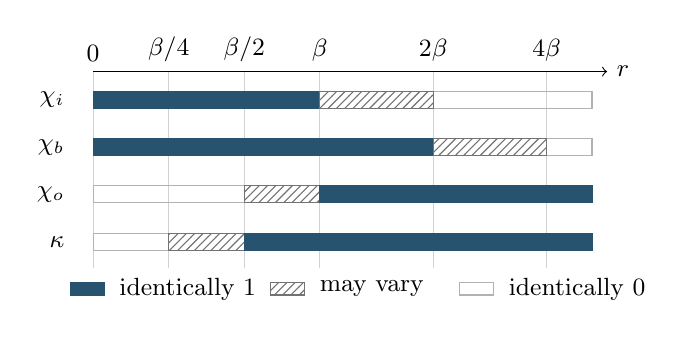
\begin{tikzpicture}[x=.96cm,y=.6cm,font=\small]
\definecolor{cutone}{RGB}{40,83,111}
\tikzset{oneregion/.style={fill=cutone,draw=cutone},
 transition/.style={pattern=north east lines,pattern color=black!55,draw=black!55}}
\foreach \x/\lab in {0/0,1/{\beta/4},2/{\beta/2},3/{\beta},4.5/{2\beta},6/{4\beta}} {
  \draw[black!18] (\x,.45)--(\x,4.6);
  \node[above] at (\x,4.6) {$\lab$};
}
\draw[->] (0,4.6)--(6.8,4.6) node[right] {$r$};
\foreach \yy/\lab in {4/{\chi_i},3/{\chi_b},2/{\chi_o},1/{\kappa}} {
 \draw[black!30] (0,\yy-.18) rectangle (6.6,\yy+.18);
 \node[left] at (-.25,\yy) {$\lab$};
}
\filldraw[oneregion] (0,3.82) rectangle (3,4.18);
\filldraw[transition] (3,3.82) rectangle (4.5,4.18);
\filldraw[oneregion] (0,2.82) rectangle (4.5,3.18);
\filldraw[transition] (4.5,2.82) rectangle (6,3.18);
\filldraw[transition] (2,1.82) rectangle (3,2.18);
\filldraw[oneregion] (3,1.82) rectangle (6.6,2.18);
\filldraw[transition] (1,.82) rectangle (2,1.18);
\filldraw[oneregion] (2,.82) rectangle (6.6,1.18);
\filldraw[oneregion] (-.3,-.13) rectangle (.15,.13);
\node[right] at (.22,0) {identically $1$};
\filldraw[transition] (2.35,-.13) rectangle (2.8,.13);
\node[right] at (2.87,0) {may vary};
\draw[black!30] (4.85,-.13) rectangle (5.3,.13);
\node[right] at (5.37,0) {identically $0$};
\end{tikzpicture}

\caption{The cutoff regions in \eqref{glue:cutoffs}. Distances are
schematic. Solid bands indicate the value one, blank bands the value
zero, and hatched bands the intervals where a cutoff may vary in
$[0,1]$; no shape or monotonicity of the transition is assumed.}
\label{fig:cutoffs}
\end{figure}

\begin{lemma}[Extension of the inner source]\label{glue:extension}
There is a real linear extension $\mathcal E_i:Y_\alpha\to
Y_\alpha(\R^m\times(-\infty,0))$, uniformly bounded for
$T\le\beta^4$, which equals $\chi_i f$ in flat coordinates for
$-T\le t<0$, and is supported spatially in $r\le2\beta$.
\end{lemma}

\begin{proof}
Put $f_i=\chi_i f$, view it in the flat coordinates, and extend it by
zero beyond their neighborhood.  The spatial extension is bounded
because the cutoff vanishes before the boundary of that neighborhood.
The $Y_\alpha$ norm gives a spatial $C^\alpha$ trace $f_i(-T,z)$ at
the lower time face.  Choose a smooth $\psi:[0,\infty)\to[0,1]$ equal
to one near zero and zero for arguments at least one.  For $t<-T$ set
\begin{equation}\label{glue:extension-formula}
 (\mathcal E_i f)(t,z)
 =f_i(-T,z)\,\psi\left(\frac{-t-T}{(|z|^2+\sqrt T)^2}\right).
\end{equation}
Let $b_0=(|z|^2+\sqrt T)^{1/2}$.  Wherever this expression is
nonzero,
\[
 T\le-t\le T+b_0^4,
 \qquad b_0^2\le |z|^2+\sqrt{-t}\le(1+\sqrt2)b_0^2.
\]
The ancient scale is therefore comparable to $b_0$.  The argument of
$\psi$ has bounded derivatives in spatial units $b_0$ and temporal
units $b_0^4$ on its transition region.  The trace norm, H\"older
multiplication, and scale comparability prove the required estimate
below $-T$.  Across that face the values agree.  Splitting a temporal
increment at $-T$ bounds its $\alpha/4$ H\"older quotient by the sum
of the two one-sided bounds; a spatial increment is handled by the
trace bound on comparable boxes.  This proves the full parabolic
$C^\alpha$ bound.  No time derivative of the source is required.
The construction is real, linear, and radial.  Its continuation below
$-T$ is in fact supported in $-26\beta^4\le t<-T$, though a temporal
support restriction is unnecessary for the ancient inverse.
\end{proof}

Apply Theorem~\ref{flat:inverse} to obtain
\[
 W_f=\wh D\mathcal E_i f,\qquad V_i=\chi_b W_f,
\]
where $V_i$ is regarded as a function on the sphere and extended by
zero.  Invariant norm equivalence and the cutoff bounds give
$\norm{V_i}_{X_\alpha}\le C\norm{f}_{Y_\alpha}$.  Define
\begin{equation}\label{glue:inner-errors}
 R_i f=(\Pcal-\wh\Pcal)(\chi_bW_f),\qquad
 J_i f=[\wh\Pcal,\chi_b]W_f.
\end{equation}
Both expressions are taken in the common coordinates and extended by
zero.  Since $\chi_b f_i=f_i$, the exact identity is
\begin{equation}\label{glue:inner-identity}
 \Pcal V_i=f_i+R_i f+J_i f.
\end{equation}
Lemma~\ref{glue:background} and $b\le C\beta$ on the relevant boxes
give
\begin{equation}\label{glue:inner-error-bounds}
 \norm{R_i f}_{Y_\alpha}\le C\beta^2\norm{f}_{Y_\alpha},
 \qquad
 \norm{J_i f}_{Y_\alpha}\le C\norm{f}_{Y_\alpha}.
\end{equation}
Here $R_i f$ is supported in $r\le4\beta$, and $J_i f$ in
$2\beta\le r\le4\beta$.  The commutator has order at most three;
on its support $b$ is comparable to $\beta$, so every derivative of
$\chi_b$ is uniformly bounded in scale units.  The definition of
$R_i$ includes the mismatch applied to the cutoff itself, and hence
accounts for all mixed cutoff and mismatch terms.

\subsection{The outer Cauchy problem and the exact right inverse}

Set
\[
 s_\beta=\max(\beta,r),\qquad \eta=T/\beta^4,
\]
and use the nonsingular weighted spaces with scale $s_\beta$.
Equivalently one can use the smooth comparable scale
$(\beta^2+r^2)^{1/2}$; the norms and all following estimates are
uniformly equivalent.  Define a modified operator on the entire sphere
by
\begin{equation}\label{glue:modified-operator}
 \Pcal_\beta=\partial_t+A_\beta\A+B_\beta,
 \qquad
 A_\beta=\kappa A_c+(1-\kappa),\qquad B_\beta=\kappa B_c.
\end{equation}
Its principal multiplier is bounded above and below by positive
constants, and $\Pcal_\beta=\Pcal$ for $r\ge\beta/2$.
Lemma~\ref{glue:background} shows, for every $j,k$, uniform bounds for
the derivatives of $A_\beta$ and $s_\beta^4B_\beta$ in units
$(s_\beta,s_\beta^4)$, with the scale fixed at the center of each box.
On the transition annulus $r\asymp\beta$ these are exactly its scaled
background bounds and the cutoff bounds.  Inside $r\le\beta/4$ the
coefficients are $1$ and $0$; outside the transition they are the
original coefficients with $\sigma\asymp s_\beta$.  The sphere
coefficients of $\A$ also have uniform bounds in these units.  These
facts verify all coefficient and ellipticity hypotheses of
Lemma~\ref{ana:short}, uniformly for $\eta\le1$.

The outer source is
\begin{equation}\label{glue:outer-source}
 f_o=f-f_i-J_i f.
\end{equation}
It vanishes for $r<\beta$ and has
\begin{equation}\label{glue:outer-source-bound}
 \norm{f_o}_{Y_\alpha(s_\beta)}\le C\norm{f}_{Y_\alpha}.
\end{equation}
Indeed $s_\beta\asymp\sigma$ on its support and on every sufficiently
small box meeting that support.  The latter assertion follows from
the Lipschitz bound for $r$ and the box radius $a_0\sigma$; it also
handles boxes crossing a support boundary.  The same comparison holds
for outputs supported in $r\ge\beta/2$.

For each fixed $\beta,T$, solve the closed-manifold Cauchy problem
\begin{equation}\label{glue:outer-cauchy}
 \Pcal_\beta Z_o=f_o,\qquad Z_o(-T)=0.
\end{equation}
The modified coefficients extend smoothly to $t=0$ by
\eqref{glue:outer-expansion}, and $f_o$ extends H\"older continuously
there: for fixed $\beta$ its nonsingular weighted norm is an ordinary
H\"older bound on a compact cylinder.  Thus the solvability assertion
in Lemma~\ref{ana:short} applies, or one may solve on truncated
cylinders and use its uniform bounds.  Uniqueness makes $Z_o$ invariant
and the solution operator real linear.

Choose a fixed $\eta_0>0$ small enough for Lemma~\ref{ana:short}
at both exponents $\alpha$ and $\alpha'$.  That Lemma gives, for
$0<\eta\le\eta_0$,
\begin{align}
 \norm{Z_o}_{X_\alpha(s_\beta)}
   &\le C\norm{f_o}_{Y_\alpha(s_\beta)},\label{glue:outer-bound}\\
 \sup s_\beta^{-p_0}\abs{Z_o}
   &\le C\eta\norm{f_o}_{Y_\alpha(s_\beta)}.\label{glue:outer-sup}
\end{align}
The constants are uniform in $\beta,T$ by the coefficient and scale
bounds verified above.  The small parameter in Lemma~\ref{ana:short}
is precisely $\eta=T/\beta^4$, since $\inf s_\beta=\beta$.
That lemma applies to zero initial data even when $f_o(-T)$ is nonzero.

Put $V_o=\chi_o Z_o$.  On the support of this product the coefficients
have already become those of $\Pcal$, and $\chi_o f_o=f_o$.
Consequently
\begin{equation}\label{glue:outer-identity}
 \Pcal V_o=f_o+J_o f,\qquad
 J_o f=[\Pcal_\beta,\chi_o]Z_o.
\end{equation}
This commutator is supported in $\beta/2\le r\le\beta$ and involves
spatial derivatives of $Z_o$ of order at most three.  For these
derivatives, Lemma~\ref{ana:interpolation} and
\eqref{glue:outer-bound}--\eqref{glue:outer-sup} give the scaled
parabolic $C^\alpha$ bound
$C\eta^{(1-\alpha)/4}\norm{f_o}_{Y_\alpha(s_\beta)}$.
Since $s_\beta\asymp\sigma\asymp\beta$ on the commutator annulus,
\begin{equation}\label{glue:outer-error-small}
 \norm{J_o f}_{Y_\alpha}
 \le C\eta^{(1-\alpha)/4}\norm{f}_{Y_\alpha}.
\end{equation}
In particular, no fourth derivative needs to be made small for this
commutator estimate.

\begin{proposition}[Uniform compact right inverse]\label{glue:inverse}
There are $\beta_0,\eta_0,C_D>0$ such that, for
$0<\beta\le\beta_0$ and $0<T\le\eta_0\beta^4$, the operator
$\Pcal$ has a real invariant right inverse
$D:Y_\alpha\to X_\alpha$ with $\norm D\le C_D$.
No initial value is prescribed for $Df$.
\end{proposition}

\begin{proof}
Define
\[
 D_{\mathrm{app}}f=V_i+V_o,\qquad \mathcal R=R_i+J_o.
\]
Equations~\eqref{glue:inner-identity}, \eqref{glue:outer-source}, and
\eqref{glue:outer-identity} give the exact operator identity
\begin{equation}\label{glue:parametrix}
 \Pcal D_{\mathrm{app}}=I+\mathcal R,\qquad
 \norm{D_{\mathrm{app}}}_{Y_\alpha\to X_\alpha}\le C,\qquad
 \norm{\mathcal R}_{Y_\alpha\to Y_\alpha}
 \le C\bigl(\beta^2+\eta^{(1-\alpha)/4}\bigr).
\end{equation}
Choose $\beta_0$ and then $\eta_0$ small enough that the last bound is
at most $1/2$ throughout the asserted range, decreasing the earlier
$\eta_0$ if necessary.  The convergent Neumann series defines
\begin{equation}\label{glue:neumann}
 D=D_{\mathrm{app}}(I+\mathcal R)^{-1}.
\end{equation}
It satisfies $\Pcal D=I$, is real and invariant, and has uniform norm
at most twice the bound for $D_{\mathrm{app}}$.  This is a right inverse
construction and requires no assertion of injectivity.
\end{proof}

\subsection{Smallness of the corrected error}

The right inverse need not have small norm.  What is needed for the
nonlinear problem is its small value on the particular error $E_c$ in
the weaker space $X'_\alpha$.

\begin{lemma}\label{glue:special-error}
For the right inverses of Proposition~\ref{glue:inverse},
\begin{equation}\label{glue:DE-small}
 \norm{DE_c}_{X'_\alpha}
 \le C\left(\beta^{2-2\delta}
       +\eta^{(\alpha'-\alpha)/4}
       +\eta^{(1-\alpha)/4}\right).
\end{equation}
In particular this norm becomes arbitrarily small by choosing $\beta$
and then $\eta=T/\beta^4$ sufficiently small.
\end{lemma}

\begin{proof}
Use the inner output cutoff, rather than the inner input cutoff, to
split
\[
 E_c=f_c+f_e,\qquad f_c=\chi_bE_c,\qquad f_e=(1-\chi_b)E_c.
\]
Equation~\eqref{glue:core-error-small} gives
$\norm{Df_c}_{X_\alpha}\le C\beta^{2-2\delta}$.
The remaining source vanishes for $r\le2\beta$, so
$\chi_i f_e=0$ exactly.  Its inner extension, flat correction,
$R_i f_e$, and $J_i f_e$ all vanish.  Thus
$D_{\mathrm{app}}f_e$ consists solely of the outer zero-data solution
for source $f_e$, followed by multiplication by $\chi_o$, and
$\mathcal R f_e=J_o f_e$.

The extra regularity in Lemma~\ref{glue:background} gives
\begin{equation}\label{glue:outer-error-high}
 \norm{f_e}_{Y_{\alpha'}(s_\beta)}\le C.
\end{equation}
The constant is uniform in $\beta,T$: in the transition annulus all
cutoff derivatives have bounded scaled size, and elsewhere this is
\eqref{glue:error-weight} or the fixed exterior smooth bound.
Apply Lemma~\ref{ana:short} at exponent $\alpha'$ to the outer
zero-data problem with source $f_e$.  The coefficient bounds hold at
that exponent, so its solution has uniformly bounded
$X_{\alpha'}(s_\beta)$ norm.  Equation~\eqref{ana:fourth-small} of
Lemma~\ref{ana:interpolation} gives an $X'_\alpha(s_\beta)$ bound
of $C\eta^{(\alpha'-\alpha)/4}$.  Multiplication by $\chi_o$ is
bounded in these scaled spaces, and $s_\beta$ is comparable to
$\sigma$ on the output support.  This proves the first estimate below;
the commutator bound \eqref{glue:outer-error-small} proves the second:
\begin{equation}\label{glue:app-special-small}
 \norm{D_{\mathrm{app}}f_e}_{X'_\alpha}
 \le C\eta^{(\alpha'-\alpha)/4},\qquad
 \norm{\mathcal Rf_e}_{Y_\alpha}
 \le C\eta^{(1-\alpha)/4}.
\end{equation}
The first estimate includes the temporal H\"older seminorms of all
spatial derivatives through order four, as supplied by
\eqref{ana:fourth-small}.  It makes no claim that the first time
derivative is small: the outer zero-data solution has time derivative
$f_e$ at the initial face.

Finally, \eqref{glue:neumann} gives
$D(I+\mathcal R)=D_{\mathrm{app}}$, so
\begin{equation}\label{glue:special-neumann-identity}
 Df_e=D_{\mathrm{app}}f_e-D\mathcal Rf_e.
\end{equation}
The uniform bound for $D$ and
\eqref{glue:app-special-small} prove the desired estimate for $f_e$.
Combining it with the estimate for $f_c$ proves
\eqref{glue:DE-small}.
\end{proof}

\subsection{The nonlinear correction and finite-time obstruction}

\begin{proof}[Proof of Theorem~\ref{glue:solution}]
Expanding \eqref{glue:equation} at $F$ gives
\begin{equation}\label{glue:nonlinear-equation}
 \Pcal V+E_c+N(V)=0,
\end{equation}
where
\begin{equation}\label{glue:nonlinearity}
 N(V)=v_*^2V^2\A F+
       \bigl(2v_*g_cV+v_*^2V^2\bigr)\A V.
\end{equation}
This expression contains only spatial derivatives of $V$, so is
defined on $X'_\alpha$.  For clarity, on a box of scale $b$, a
function with $\norm{V}_{X'_\alpha}\le\eps$ has scaled sizes
\[
 V=O(\eps b^{-2+2\delta}),\qquad
 \A V=O(\eps b^{-6+2\delta}),
\]
where these statements include the scaled parabolic $C^\alpha$
norms.  By Lemma~\ref{glue:background}, the two quadratic terms in
\eqref{glue:nonlinearity} therefore have size
$C\eps^2b^{-6+4\delta}$, and the cubic term has size
$C\eps^3b^{-6+6\delta}$.  Relative to the $Y$ weight these gain
$b^{2\delta}$ and $b^{4\delta}$, respectively.  Since $b$ is bounded
above on the compact domain, H\"older multiplication and the
factorization of differences of products give uniform bounds
\begin{align}
 \norm{N(V)}_{Y_\alpha}&\le C_N(\eps^2+\eps^3),
 \label{glue:nonlinear-size}\\
 \norm{N(V)-N(W)}_{Y_\alpha}
 &\le C_N(\eps+\eps^2)\norm{V-W}_{X'_\alpha}
 \label{glue:nonlinear-lipschitz}
\end{align}
on the closed ball of radius $\eps$ in $X'_\alpha$.  The fixed sphere
coefficients in $\A$ have bounded rescaled norms, so these estimates
apply on the whole sphere, including the other endpoint $x=1$.

We specify the parameter choices to avoid a dependence on an inverse
norm that is still being chosen.  First fix the profile, exponents,
flat inverse, and the constants $\beta_0,\eta_0,C_D$ of
Proposition~\ref{glue:inverse}.  The nonlinear constant $C_N$ is
uniform throughout this parameter range.  Choose the requested ball
radius $\eps>0$ so small that
\[
 C_D C_N(\eps+\eps^2)\le\tfrac14,\qquad
 C_*\eps\le\tfrac12\mu,
\]
where $C_*$ bounds $\abs{v_*V}/\norm{V}_{X'_\alpha}$ uniformly.
Such a $C_*$ exists because $v_*V$ has scaled size
$C\eps b^{2\delta}$ and $b\le\sqrt2$.
Now take $\beta\le\beta_0$ sufficiently small, and next
$\eta\le\min(\eta_0,a_0^4)$ sufficiently small, that
Lemma~\ref{glue:special-error} gives
$\norm{DE_c}_{X'_\alpha}\le\eps/2$; put $T=\eta\beta^4$.

The map
\[
 \mathcal T(V)=-DE_c-DN(V)
\]
takes the closed $X'_\alpha$ ball of radius $\eps$ into itself by
\eqref{glue:nonlinear-size}, and is a contraction by
\eqref{glue:nonlinear-lipschitz}.  The real invariant subspace is
closed, so the Banach fixed point theorem gives a real invariant
fixed point there.  Its fixed point identity also shows that this
same $V$ belongs to $X_\alpha$, because $E_c+N(V)\in Y_\alpha$ and
$D:Y_\alpha\to X_\alpha$.  Applying $\Pcal D=I$ therefore yields
\eqref{glue:nonlinear-equation} in the classical H\"older sense and
proves \eqref{glue:equation}.  This recovers the time derivative after
the contraction has been performed.

By \eqref{glue:background-positive} and the radius choice,
\[
 \tfrac12\mu\le 1+v_*(F+V)\le M+\tfrac12\mu,
\]
which proves \eqref{glue:positive}.  On each compact time subinterval
of $(-T,0)$, the weight is bounded above and below, and the equation
for $H$ is a uniformly parabolic scalar equation with principal
multiplier $(1+v_*H)^2$.  Its current regularity is
$C^{4+\alpha,1+\alpha/4}$.  Interior spatial difference quotients in
this equation have the same principal operator; their sources are
bounded in $C^\alpha$ because the coefficient is a smooth function
of $x,H$ and $H$ already has four spatial derivatives.  The interior
estimate of Lemma~\ref{ana:schauder}, followed by passage to the
difference-quotient limit on a smaller cylinder, gains one spatial
derivative.  Repetition gains every spatial derivative.  The equation
then gives corresponding spatial bounds for $H_t$; differentiating
the equation in time and repeating the interior estimates gives all
mixed derivatives.  Thus $H$ is smooth on $\Sigma\times(-T,0)$.
Invariant smoothness gives smoothness in $x\in[0,1]$ by
Lemma~\ref{geo:operators}.  At $x=0$, the $X'$ weight reads
\[
 \abs{V(t,0)}\le\eps\sigma(t,0)^{-2+2\delta}
                =\eps\rho^{-1+\delta},
\]
up to the fixed equivalent-norm constant.  This proves
\eqref{glue:center} and finishes the construction.
\end{proof}

\begin{proof}[Proof of Theorem~\ref{thm:main}]
Apply Theorem~\ref{glue:solution} to the nonconstant profile of
Theorem~\ref{prof:profile}.  Proposition~\ref{geo:reduction} turns
the smooth positive coefficient $H$ into a Calabi flow in the
Fubini--Study class on $\CP^{10}$.  Choose its slice at $t=-T/2$ as
the initial metric and translate time so that this slice has time
zero.  It is a smooth K\"ahler metric in a class containing the
Fubini--Study metric.  At the distinguished point,
\[
 H(t,0)=\rho^{-1}G'(0)+O(\rho^{-1+\delta}),\qquad G'(0)<0.
\]
Lemma~\ref{geo:obstruction} shows that the maximal smooth existence
time is exactly $T_*=T/2$ and that, in the elapsed time $\tau$,
\[
 S(\omega(\tau))(p)\sim a(T_*-\tau)^{-1/2},\qquad
 a=-110G'(0)>0.
\]
The metric is $U(10)$ invariant by the radial reconstruction.
These are all the assertions of Theorem~\ref{thm:main}.
\end{proof}

\begin{proof}[Proof of Corollary~\ref{cor:product-singularities}]
For a product metric the determinant factors and the inverse is block
diagonal, so scalar curvatures add.  The product volume form also shows
that their averages add.  Writing \(c_\eta=S(\eta)\), we obtain
\[
 S(\Omega(t))=\pi_X^*S(\omega(t))+c_\eta,
 \qquad \bar S_\Omega=\bar S_\omega+c_\eta.
\]
Thus \(\pi_X^*\phi(t)\), initially zero, satisfies
\eqref{eq:calabi-flow} for \(\Omega_0\).  Smooth local
uniqueness~\cite[Theorem~3.2]{ChenHe2008} identifies this explicit
solution with the unrestricted flow on \([0,T_*)\).  The displayed
scalar-curvature identity gives the stated asymptotic.  A smooth
extension across \(T_*\) would have bounded scalar curvature on the
compact product, so the maximal time is exactly \(T_*\).

For the final assertion put \(m=n-10\).  When \(m>0\), choose
\(Y=\CP^m\) and \(\eta=\frac{m+1}{11}\omega_{\mathrm{FS},m}\).
In our normalization,
\(\operatorname{Ric}(\omega_{\mathrm{FS},j})
=(j+1)\omega_{\mathrm{FS},j}\).  Constant scaling leaves the Ricci
form unchanged, so \(\omega_{\mathrm{FS},10}\) and \(\eta\) both
have Einstein constant \(11\).  Their product form is therefore
K\"ahler--Einstein and lies in \([\Omega_0]\).
For \(m=0\), use Theorem~\ref{thm:main} itself, with the second
factor a point.
\end{proof}

\appendix
\section{Certification of the finite shooting calculation}
\label{cert:appendix}
\label{sec:certificate}
\label{cert:section}

This Appendix proves the finite part of the shooting argument.  The calculation
uses integer interval arithmetic, Taylor expansion on complex disks, and a
separate estimate for the nonlinear dependence on the shooting parameters.
Every terminating decimal in this Appendix denotes its exact rational value.

\begin{proposition}[Finite shooting bounds]\label{cert:shoot}
For every parameter \(z_*\in[-R,R]^2\), where \(R=5\cdot10^{-10}\), let
\((k,d)\) be given by \eqref{prof:parameters}, and let \(p\) be the origin
solution of \eqref{prof:ode} supplied by Lemma~\ref{prof:origin}.
This solution extends to \(0\le s\le S_0=56\) and satisfies
\[
 1+p(s)>0.
\]
For the coordinates of its jet relative to \(p_{\rm a}\), defined in
\eqref{prof:coordinates}, one has
\begin{equation}\label{cert:conclusion}
 |q|\le .25R,\qquad
 \big\|(\Re\xi,\Im\xi)-z_*\big\|_\infty\le .13R.
\end{equation}
\end{proposition}

The proof compares the entire family of shots with a sequence of
reference trajectories at the central parameter \(d=d_0\).  The state
is \((p,p',p'',d)\), with \(d'=0\).  We divide \([1,56]\) into finitely
many blocks.  On each block, the reference trajectory is the exact
solution starting from a rounded three-component jet at its left
endpoint.  At the right endpoint, an interval enclosure supplies the
rounded starting jet for the next block.  Thus successive reference
trajectories may have small jumps at block boundaries; their size is
included in the error estimate.

The interval calculation encloses the reference endpoint jets and
the first-variation matrices of the four-component state across each
block.  Products of these matrices give a linear prediction for the
effect of the two shooting parameters through all blocks.  Rounding the reference jets
and variation matrices introduces separate errors.  A perturbation
estimate compares products of the rounded variation matrices with
the exact transfers and bounds the propagation of those errors.
The origin series supplies the initial central jet, its two parameter
variations, and a bound for the nonlinear parameter remainder.

It remains to compare these linear predictions with the actual
solutions for every \(z_*\in[-R,R]^2\).  The only nonlinear term in the
state equation depends on \(p\); its remainder after linearization
is quadratic in the difference from the reference value.  A uniform
bootstrap bounds this remainder using the certified positive lower
bounds for \(1+p\) along the reference trajectories and the transfer estimates.
It proves continuation and positivity for the whole shooting family and bounds its endpoint
error.  Projecting the endpoint jets into the matching coordinates
then gives \eqref{cert:conclusion}.

We use the maximum norm on vectors and the induced maximum row-sum
norm on matrices, including rectangular matrices.  For a
\(4\times4\) matrix, its superscript \((3)\) denotes its leading
\(3\times3\) block.  We first describe the interval arithmetic and
the series recurrences, then justify their analytic enclosures and
the separate nonlinear comparison.

\subsection{Integer intervals and the two series recurrences}
\label{cert:arithmetic}

Put \(Q_{\rm int}=2^{256}\).  An integer pair \((a,b)\) represents the closed
interval \([a/Q_{\rm int},b/Q_{\rm int}]\).  All arithmetic in
\texttt{verification/certificate.py} is integer arithmetic.  Addition and
multiplication by an integer are exact, with endpoint reversal for a negative
multiplier.  For multiplication, let \(m\) and \(M\) be the minimum and maximum
of the four products of integer endpoints.  The output pair is
\[
 \left(\left\lfloor\frac{m}{Q_{\rm int}}\right\rfloor,
       \left\lceil\frac{M}{Q_{\rm int}}\right\rceil\right).
\]
For a same-sign interval \((a,b)\) excluding zero, the reciprocal pair is
\[
 \left(\left\lfloor\frac{Q_{\rm int}^2}{b}\right\rfloor,
       \left\lceil\frac{Q_{\rm int}^2}{a}\right\rceil\right).
\]
These formulas are valid also for negative intervals.  Division by a positive
integer rounds each endpoint outward in the same way.  Python's integer
division is floor division, so the identity
\(\lceil x\rceil=-\lfloor-x\rfloor\) implements the required upper roundings.
In particular, \texttt{rat(a,b)} encloses the exact rational \(a/b\).
The function \texttt{mag} bounds absolute value; the function \texttt{norm}
bounds the matrix norm specified above.

The operation \texttt{widen} enlarges an interval at each end by the upper
endpoint of a nonnegative error allowance.  The operation \texttt{mid} instead
selects the grid point
\[
 Q_{\rm int}^{-1}\left\lfloor\frac{a+b}{2}\right\rfloor.
\]
For an interval of real width \(w\), its distance from every enclosed number
is at most \(w/2+Q_{\rm int}^{-1}\).  The origin and block estimates below
explicitly charge this error; midpoint selection is never used as an
enclosure operation.

Here are the coefficient identities underlying the computation.
If \(z(\theta)=\sum_{i\ge0}z_i\theta^i\) and
\(b(\theta)=1/z(\theta)=\sum_{i\ge0}b_i\theta^i\), then
\begin{equation}\label{cert:reciprocal}
 b_0=z_0^{-1},\qquad
 b_i=-z_0^{-1}\sum_{t=1}^i z_t b_{i-t}\quad(i\ge1).
\end{equation}
Writing a dot for any one parameter variation gives, for \(i\ge0\),
\begin{equation}\label{cert:tangent-reciprocal}
 \dot b_i=-z_0^{-1}
 \left(\sum_{t=0}^i\dot z_t b_{i-t}
             +\sum_{t=1}^i z_t\dot b_{i-t}\right).
\end{equation}
The second sum is empty at \(i=0\).  In the first sum the coefficient \(b_i\)
has already been computed by \eqref{cert:reciprocal}.  This is exactly the
ordering in \texttt{recip}; it includes the variation of the constant
coefficient \(z_0\).

At the origin, write \(r=s^{3/2}\) locally and
\[
 z=1+p=1+d+kr+\sum_{i\ge2}a_i r^i.
\]
Equation~\eqref{prof:ode} gives
\begin{equation}\label{cert:origin-recurrence}
 a_i=\frac{b_{i-2}-\mathbf1_{\{i=2\}}}
 { (27/8)(i-1)(i+9)(i+10)},\qquad i\ge2,
\end{equation}
where now \(b_i\) are the coefficients of the reciprocal series in \(r\).
The loop in \texttt{origin} computes \(a_2,\ldots,a_{60}\), together with
their two variations under the parameter map \eqref{prof:parameters}.
The weights for evaluation of \(p,p',p''\) at \(s=1\) are
\[
 1,\qquad \frac{3i}{2},\qquad
 \frac{3i}{2}\left(\frac{3i}{2}-1\right).
\]
The code subtracts the constant \(1\) from \(z\) only in the zeroth state
entry, as required.

For an ordinary Taylor step, let \(\ell=1/h\) be the block length,
\(s_c\) the step's initial point, \(\theta=h(s-s_c)\), and
\(\mathfrak r=hs_c+\theta\).  The equation for \(z=1+p\), with
\(E=1+d\), is
\begin{equation}\label{cert:scaled-ode}
 4\mathfrak r^3 z_{\theta\theta\theta}
 +120\mathfrak r^2 z_{\theta\theta}
 +751\mathfrak r z_\theta-1215(z-E)
 =\frac{4}{h^3}\mathfrak r^3(z^{-1}-1).
\end{equation}
This identity also gives the four tangent equations upon differentiation.
For completeness, put \(\mathfrak R=8hs_c\) and
\(F_i=b_i-\mathbf1_{\{i=0\}}\), with negative-index coefficients zero.
The scalar coefficient update used in \texttt{evolve} is
\begin{align}
 4(i+1)(i+2)(i+3)\mathfrak R^3z_{i+3}
 ={}&\frac4{h^3}\sum_{a=0}^3
     c_a\mathfrak R^{3-a}F_{i-a}\notag\\
 &-(96i+960)\mathfrak R^2(i+1)(i+2)z_{i+2}\notag\\
 &-64\mathfrak R(i+1)
       \bigl(12i(i-1)+240i+751\bigr)z_{i+1}\notag\\
 &-512\bigl(4i(i-1)(i-2)+120i(i-1)+751i-1215\bigr)z_i\notag\\
 &-1215\cdot512E\mathbf1_{\{i=0\}},
 \qquad(c_0,c_1,c_2,c_3)=(1,24,192,512).
 \label{cert:step-recurrence}
\end{align}
Indeed \(c_a\mathfrak R^{3-a}\) are the coefficients of
\((\mathfrak R+8\theta)^3\).  The initial three coefficients are
\(z_0,z_\theta(0),z_{\theta\theta}(0)/2\).
For a tangent column one differentiates every term of
\eqref{cert:step-recurrence}; the constant \(E\) has variation \(0,0,0,1\)
in the four columns.  Thus the same update computes both state and tangent
coefficients.  The values \(i=0,\ldots,43\) produce coefficients through
degree \(46\).  Horner evaluation at \(\theta=1/8\), after the appropriate
one or two differentiations, evaluates the three state entries through
degrees \(46,45,44\), respectively.  The analytic justification for their
common remainder allowance is given in Subsection~\ref{cert:disks}.

\subsection{The complete error at the origin}\label{cert:origin-error}

The parameter family of Lemma~\ref{prof:origin} is holomorphic on the
complex polydisc
\[
 |k-k_0|\le .1,\qquad |d-d_0|\le .1,
\]
and its coefficients satisfy
\begin{equation}\label{cert:origin-majorant}
 \sum_{i\ge1}|a_i|3^i<.8,\qquad a_1=k.
\end{equation}
One can check the constants directly from
\eqref{cert:origin-recurrence}: the nonfree denominators exceed \(440\),
\(3|k|<.585\), and \(|1+d|>1.30\).  The majorant improves itself because
\[
 .585+\frac9{440}\left(1+\frac1{1.30-.8}\right)
 =\frac{711}{1100}<.8.
\]
The reciprocal remains nonsingular throughout this construction.
In particular the real solutions are positive up to \(s=1\).
Also \(|d|<.501\), and \eqref{cert:origin-majorant} gives
\[
 |p(1)|<.501+\frac{.8}3<.768,\quad
 |p'(1)|\le .8\max_{i\ge1}\frac{3i/2}{3^i}\le .4,\quad
 |p''(1)|\le .8\max_{i\ge1}
       \frac{(3i/2)(3i/2-1)}{3^i}<.534.
\]
In particular the uniform bound \(2\) for every jet entry is available on
the parameter polydisc.

Let
\begin{equation}\label{cert:origin-tail}
 E_{60}=.8\,\frac{(3\cdot61/2)^2}{3^{61}}
       <5.267\cdot10^{-26}.
\end{equation}
The sequence \((3i/2)^2/3^i\) decreases for \(i\ge61\).
Consequently \(E_{60}\) bounds the omitted tail of each of the three jet
entries.  Cauchy's estimate in either parameter bounds the corresponding
first derivative of this tail at the center by \(10E_{60}\).
For the matrix in \eqref{prof:parameters}, the sum of the absolute values
of all four entries, including the factor \(10^{-8}\), is
\(.01169933\).  Thus the row norm of the omitted tail of the two
\(z_*\)-variation columns is at most \(.12E_{60}\).

Each of the two original parameter displacements has absolute value at most
\(.011R\).  The multivariable Cauchy estimate, with
\(t_*=.11R\), bounds the terms of total degree at least two in the parameter
expansion of any jet entry by
\begin{equation}\label{cert:parameter-tail}
 E_{\rm par}
 =2\sum_{j\ge2}(j+1)t_*^j
 =2\bigl((1-t_*)^{-2}-1-2t_*\bigr)
 <1.816\cdot10^{-20}.
\end{equation}
The factor \(j+1\) counts the monomials of total degree \(j\) in two
parameters.

The width assertion in \texttt{origin} bounds every computed state or
variation interval by \(10^{-20}\).
Let \(U_0\in\R^3\) be the three selected state midpoints.
Let \(Z\) have their two selected variation columns in its first three
rows, and in its fourth row the exact second row of the parameter map
\eqref{prof:parameters}.  The code stores intervals containing that exact
fourth row; its matrix estimates therefore apply to this choice of \(Z\).
Combining the state midpoint error, the state and variation tails,
the two variation midpoint errors, and \eqref{cert:parameter-tail}, gives
\begin{align}
 \left\|
 \begin{pmatrix}p(1)\\p'(1)\\p''(1)\\d\end{pmatrix}
 -\begin{pmatrix}U_0\\d_0\end{pmatrix}-Zz_*
 \right\|_\infty
 &\le 5\cdot10^{-21}+E_{60}+E_{\rm par}
        +.12E_{60}R+10^{-20}R+\frac3{Q_{\rm int}}\notag\\
 &<2.316\cdot10^{-20}<2\cdot10^{-19}.
 \label{cert:initial-error}
\end{align}
The fourth component of the error is exactly zero.
All uncertainty in the interval construction of the central rational
parameters is already included in the width assertion.

\subsection{Analytic continuation and Taylor remainder on a step}
\label{cert:disks}

The 288 blocks run from \(s=1\) to \(s=56\), with the following lengths:
\[
 \begin{array}{c|c|c}
 \text{range}&\ell&\text{number of blocks}\\ \hline
 {[1,2]}&1/32&32\\
 {[2,4]}&1/16&32\\
 {[4,8]}&1/8&32\\
 {[8,56]}&1/4&192.
 \end{array}
\]
Each block consists of eight Taylor steps of length \(\ell/8\).
At every step start the interval assertions imply, for the exact reference
state,
\begin{equation}\label{cert:step-start}
 -.76<p(0)<.4,\qquad |p_\theta(0)|<.06,\qquad
 |p_{\theta\theta}(0)|<.01.
\end{equation}
Every entry in the first three rows of the four-column scaled variation
matrix has modulus less than \(6\); its fourth row is \((0,0,0,1)\).
The step schedule gives \(hs_c\ge32\).

We now justify an analytic bound on the full complex disk
\(|\theta|\le1/2\), using only these starting bounds.
On a disk where \(|p(\theta)-p(0)|\le.1\), one has
\[
 |\mathfrak r|\ge31.5,\qquad |1+p|>.14,\qquad
 |p|<.86,\qquad |p-d_0|<1.3.
\]
Let \(H_2\) be the supremum of \(|p_{\theta\theta}|\) on any smaller
concentric disk.  Integrate the equation for \(p_{\theta\theta}\)
along radial line segments and apply the integral Gronwall inequality.
Since
\[
 \frac{30}{31.5}<.954,\qquad
 \frac{B}{31.5^2}<.190,\qquad
 \frac{|C|}{31.5^3}<.011,\qquad h^{-3}\le.015625,
\]
and \(|p_\theta|\le .06+H_2/2\), this gives
\begin{equation}\label{cert:disk-h2}
 H_2\le
 e^{.954/2}\left[
 .01+\frac12\left\{.190(.06+H_2/2)
               +.011\cdot1.3+.015625\frac{.86}{.14}\right\}\right].
\end{equation}
The coefficient of \(H_2\) on the right is less than one.
Solving this linear inequality yields \(H_2<.123602<.13\).
Therefore
\begin{equation}\label{cert:disk-displacement}
 |p(\theta)-p(0)|\le .06/2+.13/8=.04625<.1.
\end{equation}
This strictly improves the bootstrap.  On every disk of radius at most
\(1/2\), the state and its first two derivatives are bounded and both
denominators \(\mathfrak r\) and \(1+p\) stay uniformly away from zero.
The local holomorphic ODE theorem then continues the solution across any
putative boundary of its disk of existence.  Uniqueness makes the
continuations agree.  Thus the solution is holomorphic on a neighborhood
of the closed disk of radius \(1/2\), with the displayed bounds.

In the scaled state \((p,p_\theta,p_{\theta\theta},d)\), the Jacobian is
\begin{equation}\label{cert:scaled-jacobian}
 \mathcal J(\theta)=
 \begin{pmatrix}
 0&1&0&0\\
 0&0&1&0\\
 -C/\mathfrak r^3-h^{-3}/(1+p)^2&
       -B/\mathfrak r^2&-30/\mathfrak r&C/\mathfrak r^3\\
 0&0&0&0
 \end{pmatrix}.
\end{equation}
On the complex disk its norm is bounded by the maximum of \(1\) and
\[
 \frac{30}{31.5}+\frac{751/4}{31.5^2}
       +\frac{1215/2}{31.5^3}+\frac{1/64}{.14^2}<2.1.
\]
Each actual variation column, with initial norm at most \(6\), consequently
has norm at most \(6e^{2.1/2}<17.146<32\) throughout the disk.
The state entries themselves also have modulus less than \(32\).
These estimates apply to the actual block variation already propagated
from the block's initial identity matrix; a new identity is not assumed
at each substep.

If a scalar holomorphic function is bounded by \(32\) on this disk,
Cauchy's coefficient estimate gives a tail after degree \(44\), at
\(\theta=1/8\), bounded by
\begin{equation}\label{cert:step-tail}
 32\sum_{i\ge45}\left(\frac{1/8}{1/2}\right)^i
 =\frac{128}{3}\,4^{-45}<48\,4^{-45}.
\end{equation}
Every state entry and every tangent entry is approximated to at least
degree \(44\).  Hence the allowance \(48\,4^{-45}\) added by
\texttt{evolve} encloses all their Taylor tails.  The interval recurrences
then inductively enclose the exact reference solution and its exact
first variation through all eight substeps.

On a real substep, the sharper displacement bound is
\begin{equation}\label{cert:real-step-displacement}
 |p(\theta)-p(0)|
 \le .06/8+\frac{.13}{2\cdot8^2}
 =.008515625<.01.
\end{equation}
Accordingly, the smallest lower starting endpoint for \(1+p\), reduced
by \((\lfloor Q_{\rm int}/100\rfloor+1)/Q_{\rm int}>.01\), is a valid
lower bound \(m_j\) on the entire reference block.  This is the variable
\texttt{mini} divided by \(Q_{\rm int}\).

\subsection{The finite inequalities and their exact interpretation}
\label{cert:ledger}

Write the block endpoints as \(s_0=1,\ldots,s_N=56\), \(N=288\).
On block \(j\), the reference solution has initial physical jet \(U_j\)
and parameter \(d_0\); it is evolved exactly on that block.
The rounded jet selected for the next block is \(U_{j+1}\).
Let \(M_j\) be the exact \(4\times4\) transfer of the linearized
four-component physical state along this reference block.

The conversion from scaled derivatives to physical derivatives is essential.
With
\[
 S_j=\diag(1,\ell_j,\ell_j^2,1),
\]
a scaled transfer \(T\) becomes \(S_j^{-1}TS_j\).
Thus its entry in row \(a\), column \(b\), for \(a,b\in\{0,1,2\}\),
is multiplied by \(h_j^a/h_j^b\); column \(3\) is multiplied by \(h_j^a\).
The fourth row remains \((0,0,0,1)\).
The code performs this conversion before asserting the widths.
Consequently its assertions imply
\begin{equation}\label{cert:local-errors}
 \big\|U_{j+1}- (p_{\rm ref},p'_{\rm ref},p''_{\rm ref})
                         (s_{j+1})\big\|_\infty<10^{-19},
 \qquad
 |(M_j-\widetilde M_j)_{ab}|<10^{-15},
\end{equation}
where \(\widetilde M_j\) is the selected matrix of transfer midpoints.
The state and transfer widths are, respectively, less than
\(10^{-19}\) and \(10^{-15}\); the stated looser midpoint bounds follow
from the midpoint estimate in Subsection~\ref{cert:arithmetic}.
All fourth-component errors in \eqref{cert:local-errors} are zero.

Define the products of these point matrices by
\[
 \widetilde T_{i,j}=
 \widetilde M_{i-1}\cdots\widetilde M_j\quad (i>j),
 \qquad \widetilde T_{i,i}=I_4.
\]
The exact integer comparisons in \texttt{check} give
\begin{align}
 m_j&>.23,\qquad \|Z\|<.02,\notag\\
 \max_{i\ge j}\|\widetilde T_{i,j}\|&\le8500,
 &\max_i\sum_{j<i}\|\widetilde T_{i,j+1}^{(3)}\|&\le570000,\notag\\
 \max_i\sum_{j<i}\frac{\ell_j}{m_j^3}
                \|\widetilde T_{i,j+1}^{(3)}\|&\le246000,
 &\max_i\|\widetilde T_{i,0}Z\|&\le2.7.
 \label{cert:finite-products}
\end{align}
Here and below a maximum over endpoints includes endpoint \(0\);
the assertion for it follows from \(\|Z\|<.02\).

To explain the summation indices, for each endpoint \(i\) the inner loop
starts with the identity and takes \(j=i-1,\ldots,0\).
Immediately before multiplying by \(\widetilde M_j\), its current interval
matrix encloses \(\widetilde T_{i,j+1}\).
The update \texttt{T=mm(T,allm[j])} therefore produces the desired forward
product in the correct order.  If \(r_j=Q_{\rm int}m_j\) and \(\mathfrak d\)
is the integer interval bound for the leading \(3\times3\) norm, then
\[
 \frac{\mathfrak d Q_{\rm int}^{\,2}}{h_jr_j^3}
 =\frac{\ell_j}{m_j^3}\frac{\mathfrak d}{Q_{\rm int}}.
\]
The expression used for \texttt{K} is its floor plus one, hence an upper
bound even when the quotient is integral.  Thus the interval product
arithmetic and the weighted sum both round in the required direction.

Let \(P_{\rm a}(d)=(p_{\rm a},p'_{\rm a},p''_{\rm a})(56)\), and put
\(Y=(\widetilde T_{N,0}Z)_{\mathrm{top}\,3}\).
The final comparisons in \texttt{check} give
\begin{align}
 \|U_N-P_{\rm a}(d_0)\|_\infty&<.04R,&
 \|\Lambda(U_N-P_{\rm a}(d_0))\|_\infty&<.006R,\notag\\
 \|(\Lambda Y)_{1,\cdot}\|_{\rm row}&<.116,&
 \|(\Lambda Y)_{\mathrm{bottom}\,2}-I_2\|&<.001.
 \label{cert:finite-matching}
\end{align}
The jet factors used for the term \(d_m s^{-3m}\) are
\(1,-3m,3m(3m+1)\), with denominators \(56^{3m}\),
\(56^{3m+1}\), \(56^{3m+2}\), respectively.
After multiplication by \(d_m\), these give its value and first two
derivatives at \(s=56\).
The index test in the last assertion subtracts the \(2\times2\) identity
from the two nonreal-coordinate rows.

The listed comparisons are finite integer statements: the displayed source
constructs their operands and asserts them.  Subsection~\ref{cert:provenance} gives the command for checking them
with assertions enabled.
The preceding recurrence and disk arguments prove that these finite
statements bound the specified analytic trajectories and variations.

\subsection{Transfer errors and estimates within a block}
\label{cert:transfer-errors}

Let \(T_{i,j}=M_{i-1}\cdots M_j\) be the exact products.
By \eqref{cert:local-errors},
\(\|M_j-\widetilde M_j\|<4\cdot10^{-15}\).
Expand a product of at most \(288\) factors, choosing the error factor at
\(k\) positions.  Each intervening, possibly empty, product of approximate
factors has norm at most \(8500\), by \eqref{cert:finite-products}.
Summing the bounds for \(k\ge1\) gives
\begin{equation}\label{cert:product-perturbation}
 \|T_{i,j}-\widetilde T_{i,j}\|
 \le8500\left[(1+4\cdot10^{-15}\cdot8500)^{288}-1\right]
 <.001.
\end{equation}
In particular \(\|T_{i,j}\|<8501\).  Since the lengths of all the
blocks sum to \(55\), \eqref{cert:finite-products} implies
\begin{equation}\label{cert:exact-sums}
 \max_i\sum_{j<i}\|T_{i,j+1}^{(3)}\|\le580000,\qquad
 \max_i\sum_{j<i}\frac{\ell_j}{m_j^3}
             \|T_{i,j+1}^{(3)}\|\le250000,
\end{equation}
using the elementary comparisons
\[
 570000+288\cdot.001<580000,\qquad
 246000+\frac{55\cdot.001}{.23^3}<250000.
\]
Also
\begin{equation}\label{cert:linear-size}
 \|T_{i,0}Z\|\le2.7+.001\cdot.02<2.72.
\end{equation}

We need two estimates for transfers between any two ordered points of
one reference block, including points in different Taylor substeps.
The real scaled Jacobian \eqref{cert:scaled-jacobian} has norm at most
\[
 L_{\rm real}=
 \max\left\{1,\frac{30}{32}+\frac{751/4}{32^2}
                  +\frac{1215/2}{32^3}
                  +\frac{1/64}{.23^2}\right\}.
\]
An interval of at most one block unit therefore has scaled transfer norm
at most \(e^{L_{\rm real}}<4.3\).
Let \(\Phi_j(s,t)\) denote its physical transfer.
Conjugation by \(S_j\) does not increase either the first-row norm or the
maximum norm of the third column: in the first row the scaling factors
are \(1,\ell_j,\ell_j^2,1\), and in the third column they are
\(\ell_j^2,\ell_j,1,\ell_j^2\).
Thus, with \(e_3=(0,0,1,0)^t\),
\begin{equation}\label{cert:partial-transfer}
 \|(\Phi_j(s,t))_{1,\cdot}\|_{\rm row}\le4.3,\qquad
 \|\Phi_j(s,t)e_3\|_\infty\le4.3
 \quad(s_j\le t\le s\le s_{j+1}).
\end{equation}
Only these two parts of a physical transfer are needed.  Its full norm
need not satisfy the same estimate.

All exponential comparisons just used, and the one in
\eqref{cert:disk-h2}, can be checked by rational arithmetic.
For \(0\le x<82\), let
\[
 E_{80}(x)=\sum_{j=0}^{80}\frac{x^j}{j!}
 +\frac{x^{81}}{81!}\frac1{1-x/82}.
\]
The positive exponential tail has successive ratios at most \(x/82\),
so \(e^x\le E_{80}(x)\).
Substituting the displayed rational values in this formula verifies all
the strict numerical comparisons.  The supplementary
\texttt{verification/arithmetic\_allowances.py} performs these rational
checks, including \eqref{cert:initial-error},
\eqref{cert:product-perturbation}, and the remaining comparisons below.

\subsection{Uniform nonlinear error and closure of the bootstrap}
\label{cert:nonlinear}

Fix \(z_*\in[-R,R]^2\).  On each block compare its actual shot with the
reference solution on that block, and write \(\delta p=p-p_{\rm ref}\).
For the only nonlinear term in the physical third-component equation,
\[
 -\frac{p}{1+p}
 +\frac{p_{\rm ref}}{1+p_{\rm ref}}
 +\frac{\delta p}{(1+p_{\rm ref})^2}
 =\frac{(\delta p)^2}{(1+p_{\rm ref})^2(1+p)}.
\]
It follows that the difference equation, beyond the reference
linearization, has forcing \(e_3\mathcal N\), where
\begin{equation}\label{cert:nonlinear-remainder}
 |\mathcal N|=
 \frac{|\delta p|^2}{|1+p_{\rm ref}|^2|1+p|}.
\end{equation}
The \(d\)-dependence is linear and is already included in the fourth
variation component.

Temporarily assume \(|\delta p|\le14R\) throughout the portions of the
blocks reached so far.  Since \(m_j>.23\) and
\(m_j/(m_j-14R)<1.001\), \eqref{cert:nonlinear-remainder} implies
\[
 |\mathcal N|\le\frac{1.001(14R)^2}{m_j^3}.
\]
The error accumulated by the end of block \(j\), before multiplication
by subsequent complete-block transfers, has zero fourth component.
Its norm is bounded by
\[
 10^{-19}
  +4.3\,\ell_j\frac{1.001(14R)^2}{m_j^3}.
\]
The first term is the reference jump
\eqref{cert:local-errors}; the second follows by variation of constants
and the third-column estimate in \eqref{cert:partial-transfer}.

Define the endpoint error \(e_i\) by
\[
 \begin{pmatrix}p(s_i)\\p'(s_i)\\p''(s_i)\\d\end{pmatrix}
 =\begin{pmatrix}U_i\\d_0\end{pmatrix}
          +T_{i,0}Zz_*+e_i.
\]
Its fourth component is zero.  By \eqref{cert:initial-error},
\eqref{cert:exact-sums}, and the preceding local error estimate,
\begin{align}
 \|e_i\|_\infty
 &\le580000\cdot10^{-19}+8501\cdot(2\cdot10^{-19})
       +4.3\cdot250000\cdot1.001(14R)^2\notag\\
 &=.1055747504R<.11R.
 \label{cert:endpoint-error}
\end{align}
For an interior point of a block, the first-row estimate in
\eqref{cert:partial-transfer}, \eqref{cert:linear-size}, and the forcing
estimate give
\begin{align}
 |\delta p|
 &\le4.3(2.72+.11)R
      +4.3\frac{1.001(14R)^2}{.23^3}\notag\\
 &<12.169035R<14R.
 \label{cert:bootstrap-improvement}
\end{align}
Here replacing the remaining block length by \(1\) is a harmless
overestimate.  This improves the bootstrap strictly both at block starts
and in block interiors, including the reference jumps.
At \(s=1\) it starts from \(\|Z\|<.02\) and
\eqref{cert:initial-error}.  Continuation over the finitely many blocks
therefore proves \eqref{cert:endpoint-error} at every block endpoint.

For clarity, existence is part of this continuation argument.
As long as the bootstrap holds, \(1+p\ge .23-14R>0\).
On the finite interval \(1\le s\le56\), the equations for \(p'\) and
\(p''\) form a linear system with bounded coefficients and bounded forcing
once \(p\) stays in this range.  Gronwall's inequality bounds these
derivatives on every such interval.  Thus no other finite-time escape
can interrupt continuation.  Positivity before \(s=1\) was established
in Subsection~\ref{cert:origin-error}.  This proves the existence and
positivity statements of Proposition~\ref{cert:shoot}.

\subsection{Projection at the matching point}\label{cert:projection}

Let \(\Gamma\) denote the exact real coordinate matrix of
\eqref{prof:coordinates}.
Lemma~\ref{prof:root-bounds} gives
\[
 |\Gamma_{ab}-\Lambda_{ab}|<.001,
 \qquad
 \|\Gamma_{1,\cdot}\|_{\rm row}<.92,\qquad
 \|\Gamma_{a,\cdot}\|_{\rm row}<.68\quad(a=2,3).
\]
Thus \(\|\Gamma-\Lambda\|<.003\).
The polynomial \(P_{\rm a}\) also satisfies
\begin{equation}\label{cert:pa-variation}
 \|P_{\rm a}(d)-P_{\rm a}(d_0)\|_\infty
 \le .01|d-d_0|\le .01\cdot.011R;
\end{equation}
this follows by differentiating the four explicit coefficients in
\eqref{prof:asymptotic-polynomial}, as detailed in the proof of
Lemma~\ref{prof:tail-residual}.

Set \(A_*=U_N-P_{\rm a}(d_0)\).
The endpoint error and transfer error give
\[
 \begin{pmatrix}p\\p'\\p''\end{pmatrix}(56)-P_{\rm a}(d)
 = A_*+Yz_*+\epsilon_*
       -\bigl(P_{\rm a}(d)-P_{\rm a}(d_0)\bigr),
 \qquad
 \|\epsilon_*\|_\infty\le
       \bigl(.11+.001\cdot.02\bigr)R.
\]
In fact \(\epsilon_*\) is the sum of the top three entries of \(e_N\)
and \(((T_{N,0}-\widetilde T_{N,0})Zz_*)_{\mathrm{top}\,3}\).
Apply one row of \(\Gamma\).
The contribution of \(A_*\), using \eqref{cert:finite-matching}, is at
most \((.006+.003\cdot.04)R\).
For the first row the linear contribution is bounded by
\((.116+.003\cdot2.7)R\).
For row \(a=2,3\), after subtracting the corresponding coordinate of
\(z_*\), it is bounded by \((.001+.003\cdot2.7)R\).
The remaining contribution is bounded by the row norm of \(\Gamma\)
times
\[
 \bigl(.11+.001\cdot.02+.01\cdot.011\bigr)R.
\]
Consequently, in units of \(R\), the two required estimates are
\begin{align*}
 |q|/R
 &\le .006+.003\cdot.04+.116+.003\cdot2.7
       +.92(.11+.001\cdot.02+.01\cdot.011)\\
 &=.2315396<.25,\\
 \big\|(\Re\xi,\Im\xi)-z_*\big\|_\infty/R
 &\le .006+.003\cdot.04+.001+.003\cdot2.7
       +.68(.11+.001\cdot.02+.01\cdot.011)\\
 &=.0901084<.13.
\end{align*}
These are exact rational comparisons and establish
\eqref{cert:conclusion}, completing the proof of
Proposition~\ref{cert:shoot}.

\subsection{Executable source and reproducibility}
\label{cert:provenance}

The complete source printed in Appendix~\ref{app:code} is
\texttt{verification/certificate.py}, comprising \(6594\) UTF-8 bytes.
Its SHA-256 digest is
\begin{center}\small\ttfamily
263389fd7217d84d0e5b66869797fc9f7998\\
309d524a95f7ad7d3d0f538ea742
\end{center}
where the line break is for typesetting only.
It uses no imported libraries, floating-point operations, external data,
or platform-dependent numerical routines.  From the paper directory,
the verification command is
\begin{quote}\ttfamily
python3 verification/certificate.py
\end{quote}
with Python assertions enabled (no \texttt{-O} or \texttt{-OO}, and no
\texttt{PYTHONOPTIMIZE} setting that disables assertions).
The program is silent when every assertion succeeds.

The supplementary rational check
\begin{quote}\ttfamily
python3 verification/arithmetic\_allowances.py
\end{quote}
verifies the analytic allowances used above by exact fraction arithmetic;
its decimal report is descriptive only.
The optional script \texttt{verification/tail-check.py} checks the explicit
root and tail estimates in Section~\ref{sec:profile} by exact rational
arithmetic.
The finite integer assertions, the analytic enclosure argument in
Subsections~\ref{cert:origin-error}--\ref{cert:disks}, and the nonlinear
argument in Subsections~\ref{cert:transfer-errors}--\ref{cert:projection}
together prove the finite shooting proposition.

\section{The exact-arithmetic certificate}\label{app:code}
The following Python program is the certificate used in
Appendix~\ref{sec:certificate}. It uses only Python's standard library and
integer arithmetic. Run it with assertions enabled. Successful termination
means that all its assertions hold; the analytic interpretation of those
assertions is proved in Appendix~\ref{sec:certificate}.
\lstinputlisting[style=certificate]{../verification/certificate.py}
\begingroup
\small
\let\originalthebibliography\thebibliography
\renewcommand{\thebibliography}[1]{%
  \originalthebibliography{#1}%
  \setlength{\itemsep}{1pt}%
  \setlength{\parsep}{0pt}%
  \setlength{\parskip}{0pt}%
}
\bibliographystyle{plain}
\bibliography{references}
\endgroup
\end{document}
